\documentclass[conference]{IEEEtran}
\usepackage{pgfplots}
\usepackage{pgfplotstable}
\usepackage{graphicx}
\usepackage{mdframed}
\pagestyle{plain}
\author{
Ben Steele \\
Colorado College\\
\texttt{Benjamin.Steele@coloradocollege.edu} \\
}
\begin{document}

\title{Iterative Resolution}

\author{\IEEEauthorblockN{Ben Steele}
\IEEEauthorblockA{Colorado College\\
Benjamin.Steele@ColoradoCollege.edu}}

\maketitle

\begin{abstract}
Resolution is a theorem proving algorithm that works with logical knowledge bases.  The algorithm works by passing through the knowledge base multiple times, resolving every clause and building up more clauses, until a contradiction is found or no more clauses can be resolved.  Generally from one pass through the clauses to the next, there is an exponential increase in the number of clauses.  We saw this as a potential issue and designed a way to withhold some clauses from the next pass, then add them to a later pass.  We found that doing this process does not change the speed of the algorithm in any significant way.
\end{abstract}
\section{Introduction}
Resolution is a fundamental algorithm in processing logic.  It can be used for theorem proving in mathematics and was an essential tool in artificial intelligence during the origin of the field.  The algorithms associated with logic are generally slow and unable to cope with large problems or large knowledge bases.  This is the reason logic based artificial intelligence has fallen out of favor and statistican algorithms have become far more favorable, expecially with big data.  Finding ways to improve the speed of logic based algorithms can help make logic more viable in the modern field of AI.  Our research aimed to increase the speed of the resolution algorithm.

\subsection{Resolution}
Resolution is a theorem proving algorithm that  uses proof by contradiction.  In order to set up a problem for resolution we must frame it using a knowledge base and a query.  A knowldege base is a collection of logical statements that define the background information for the problem.  The query is a single logical statement that we want to determine to be true or false with respect to the knowledge base. 

For any knowledge base $KB$ and query $q$, to determine if $KB$ entails $q$ we must show that $(KB \land \neg q)$ is unsatisfiable.  To show that it is unsatisfiable we find a contradiction.  If no contradiction is found, it is satisfiable and the query is flase.  In the next few paragraphs we will explain why resolution works.

A knowledge base must be converted to conjunctive normal form (CNF) before resolution can be applied to it.  CNF arranges a knowledge base into clauses joined by conjunctions.  Each clause contains literals joined by disjunctions (see example below).  Any first order logic statement can be converted into CNF.

\textbf{Example CNF:}
  $$(l_1 \lor l_2) \land (l_3 \lor \neg l_1 \lor l_4) \land (\neg l_2)$$

Once the knowledge base is in CNF we can convert the query to CNF and append its complement to the knowledge base.  We do this becuase if the complement is false, then the query must be true.  As we will see later, resolution is much faster at finding a false result than a true result, so resolving with the complement allows us to discern if the query is true faster.  Once the complement is appended, we can resolve the knowledge base to see if the complement added a contradiction.

When we consider resolution, we are concerned with satisfiability.  For a knowledge base to be satisfiable, there must be at least one assignment of literals such that the knowledge base is true.  Because CNF clauses are joined by conjunctions, satisfiability can be determined by whether there is an assingmnet such that all clauses are true.

\begin{figure}
  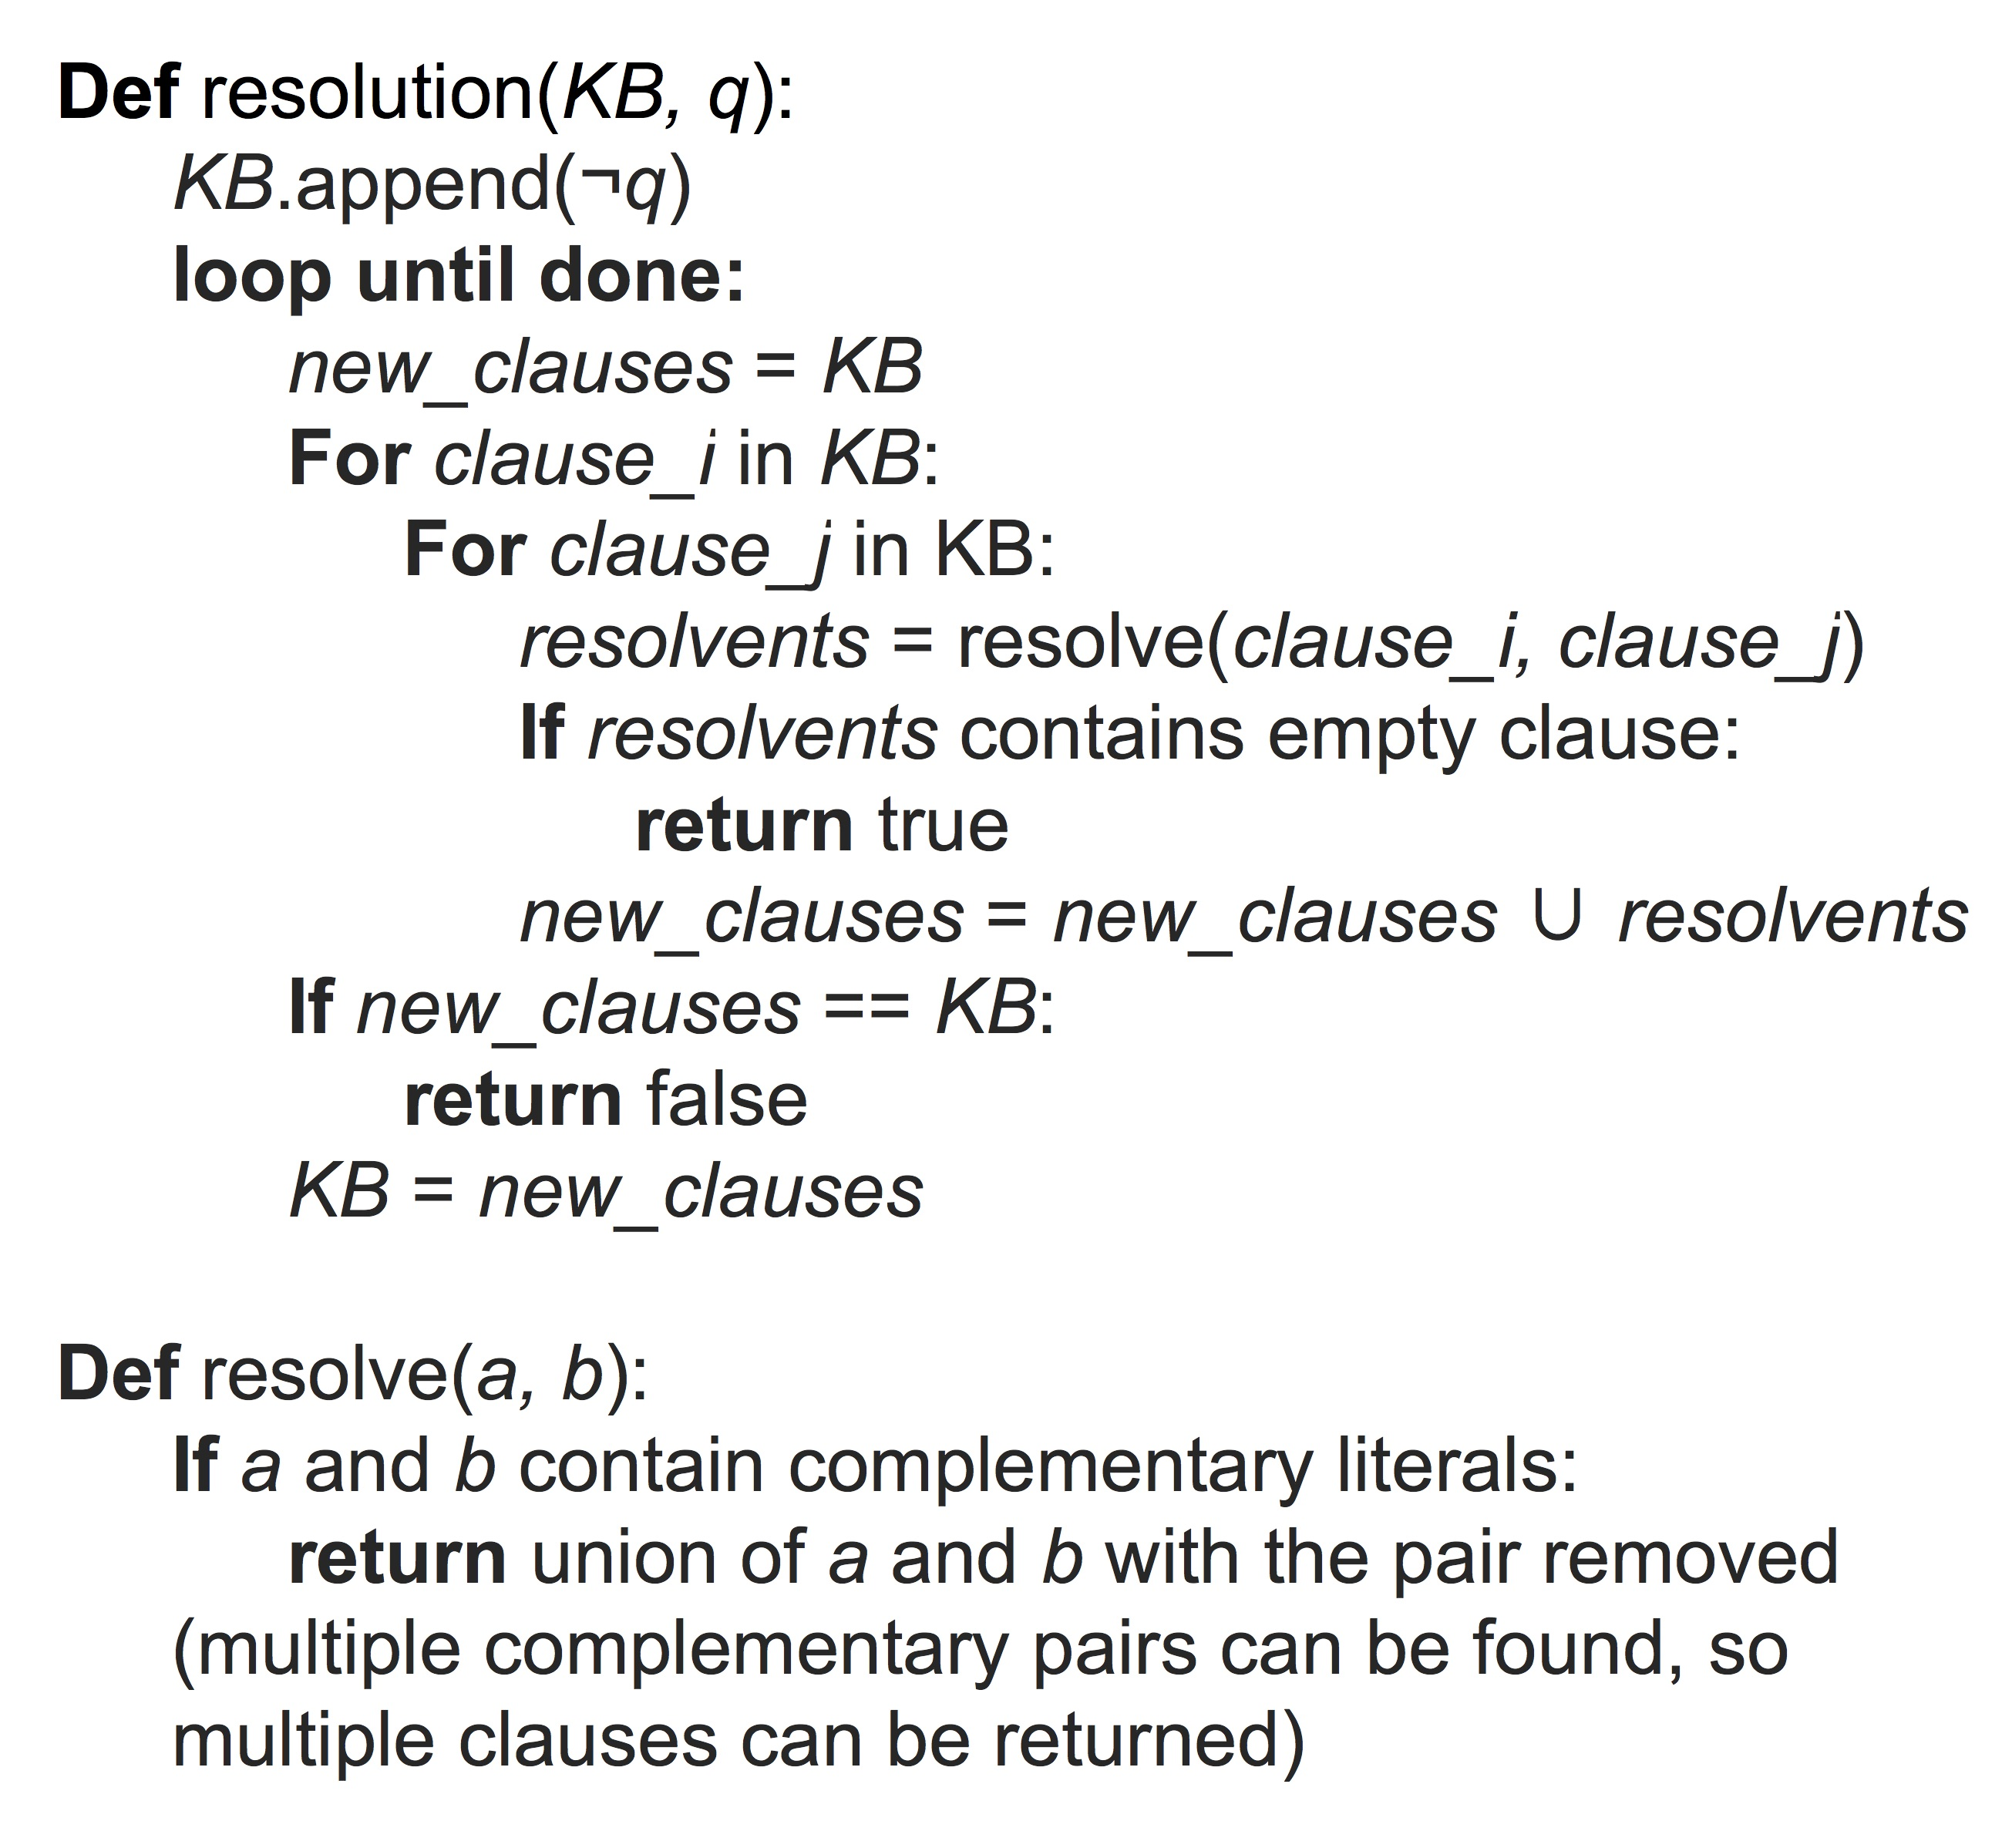
\includegraphics[scale=.1]{ResolutionCode}
  \caption{Pseudocode for the resolution algorithm taking a knowledge base (KB) and query (q) as inputs}
\end{figure}

\begin{figure*}
  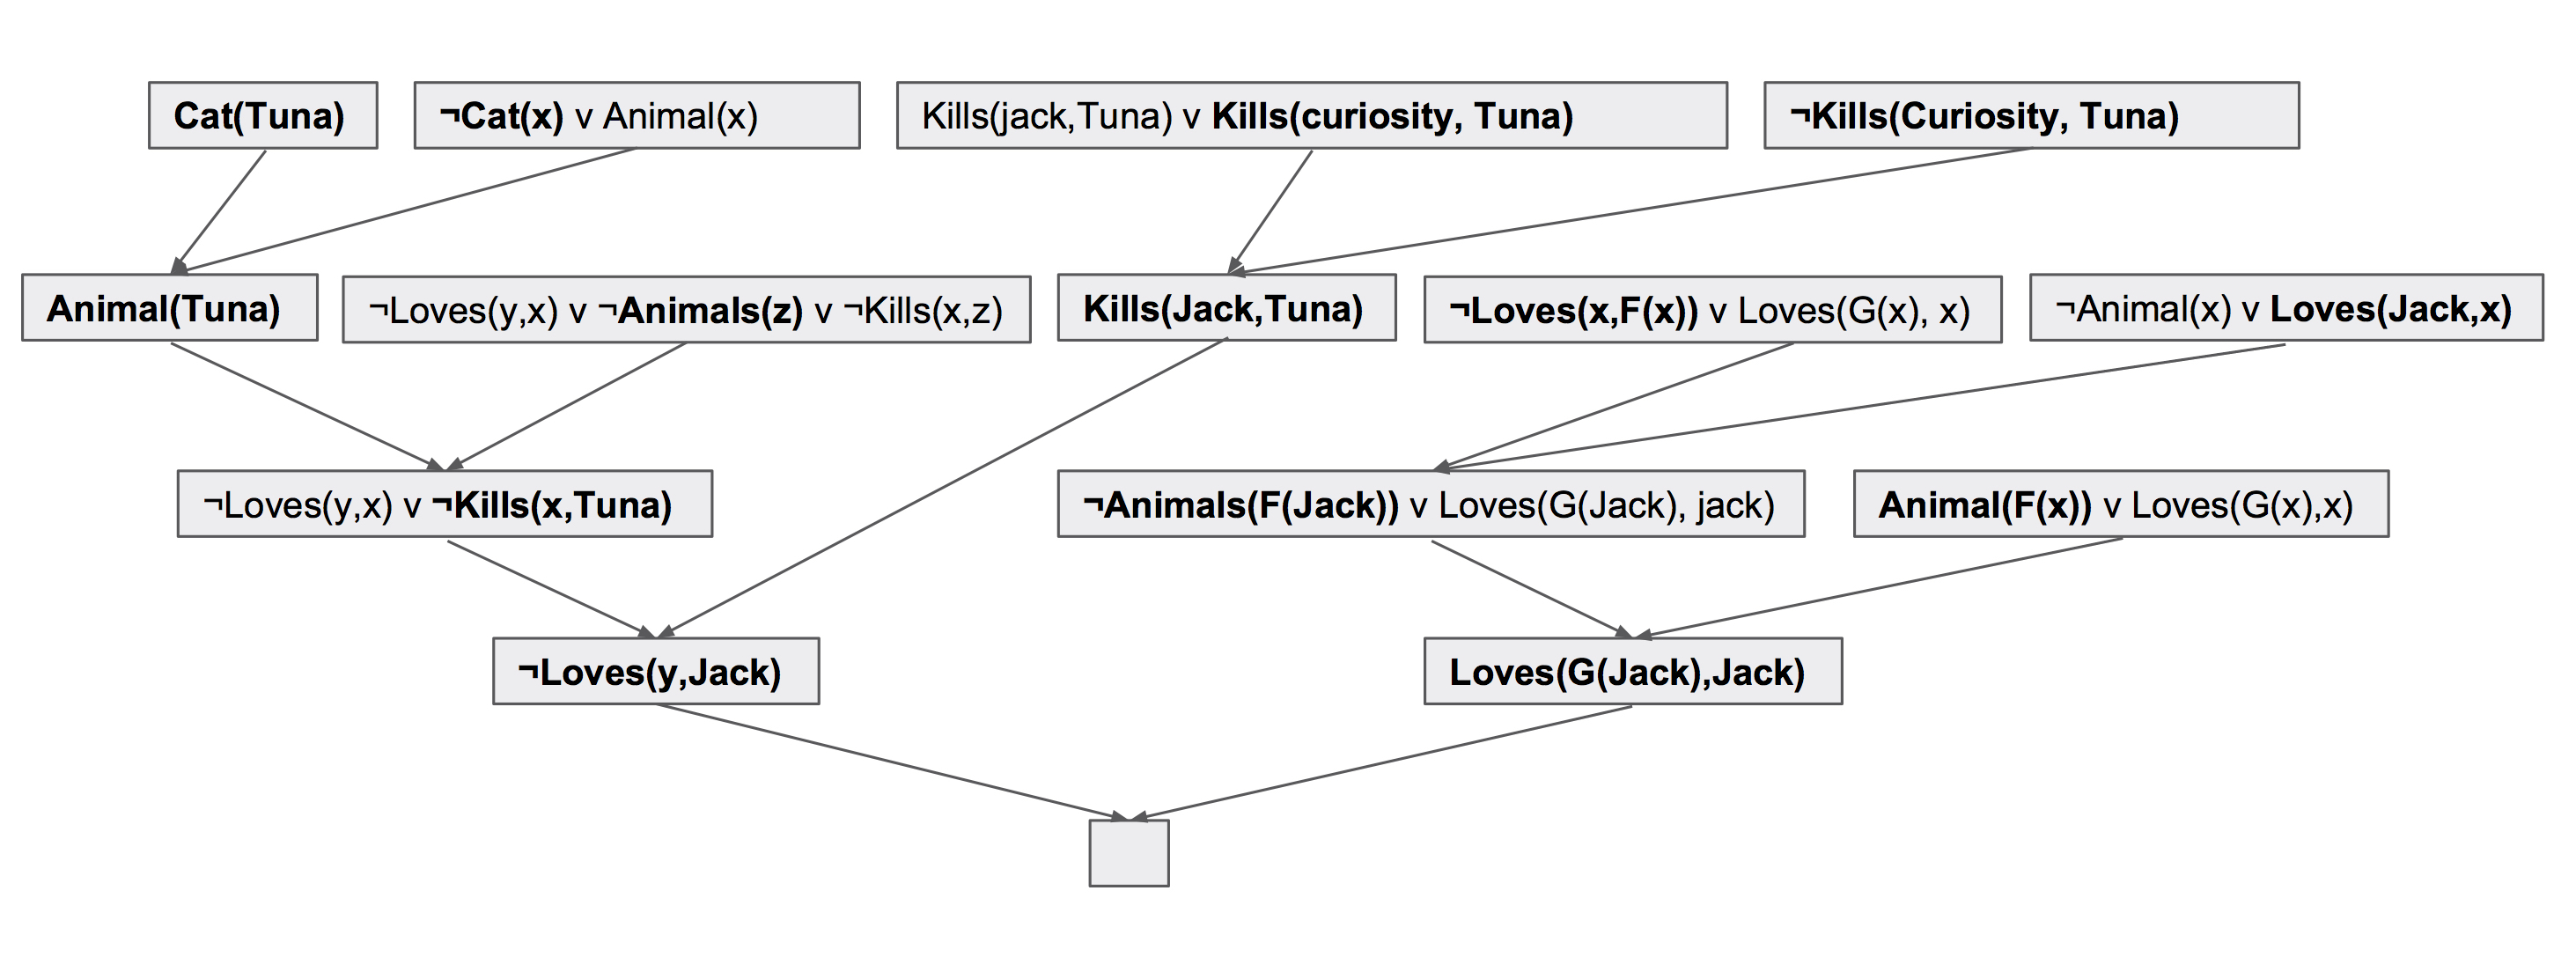
\includegraphics[width=\textwidth,height=7cm]{FOResolution}
  \caption{Here a tree of resolution is shown.  Only the clauses essential for getting to the empty clause are shown in the tree.  This resolution shows that curiosity killed the cat.  It is important to note that there are many more clauses that must be resolved that do not contribute to reaching the empty clause and are not shown in the tree.  }
\end{figure*}

\begin{figure}
  \begin{mdframed}
  \textbf{Knowledge Base:}\newline

  Everyone who loves all animals is loved by someone.
  
  Anything That kills an animal is loved by no one.

  Jack loves all animals.

  Either Jack or Curiosity killed the cat, who is named Tuna.\newline
  
  \textbf{Query:} Did Curiosity kill the cat?

  Solution in diagram above\newline
  
 \textbf{ CNF Form Clauses:}\newline

  $Animal(F(x)) \lor Loves(G(x),x)$

  $\neg Loves(x,F(x)) \lor Loves(G(x),x)$

  $\neg Loves(y,x) \lor \neg Animal(z) \lor \neg Kills(x,z)$

  $\neg Animal(x) \lor Loves(Jack,x)$

  $Kills(Jack,Tuna) \lor Kills(Curiosity,Tuna)$

  $Cat(Tuna)$

  $\neg Cat(x) \lor Animal(x)$

  $\neg Kills(Curiosity, Tuna)$
  \end{mdframed}
  \caption{Above we see the english logic statements that make up a knowledge base as well as the CNF form once the complement of the query is added.  Note that in the diagram above every CNF clause is used at some point in the resolution tree.}
\end{figure}

Suppose two clauses $a$ and $b$ each contain one of a pair of complementary literals, $l$ and $\neg l$ respectively.  This means that no matter what is assigned to $l$, it will be true in one of the clauses and false in the other.

$$a \ \ \ \ \ \ \ \ \ \ \ \ \ \ \ b$$
$$(x \lor l) \ \ \ \ \ \ \ \  (y \lor \neg l)$$

Becuase a clause is a disjunction of literals, as long as one literal is true within a clause, the clause is true.  If one of the non $l$ literals in $a$ is true we already know that the entire clause is true, so we can assign anything to $l$ and $a$ will still be true.

$$(true \lor l) = true$$

We can assign $false$ to $l$ so that $\neg l$ is true.  $b$ contains $\neg l$, which is now $true$, so  $b$ must be true as well.

$$(y \lor \neg (false)) = true$$

Therefore both clauses must be satisfiable if a non $l$ literal is true in $a$.  We can do the same for a non $l$ literal in $b$.

Because this is true whether the non $l$ literal is in $a$ or $b$, both clauses must be satisfiable if one of the non $l$ literals in either clause is true.

The key to this is that one of the non $l$ literals in either clause is true.  In logic this can be  written as a disjunction of all non $l$ literals in either clause.  This is how you resolve clauses.

For the clauses $$(k_1 \lor \cdot \cdot \cdot \lor k_n), (l_1 \lor \cdot \cdot \cdot \lor l_m)$$
If $k_i$ and $l_j$ are complementary literals, the resolved clause is $$(k_1 \lor \cdot \cdot \cdot \lor k_{i-1} \lor k_{i+1} \lor \cdot \cdot \cdot \lor k_n \lor l_1 \lor \cdot \cdot \cdot \lor l_{j-1} \lor l_{j+1} \lor \cdot \cdot \cdot \lor l_m)$$

Resolution takes two clauses and produces a new clause containing all the literals of the two original clauses except the two complementary literals.  A resolved clause has the same satisfiability as its two parent clauses, as we explained above.



Using this method of resolving clauses into a new clause we can continue to expand the number of clauses.  The resolved clause does not contain all the information of the parent clauses, so we cannot replace the parent clauses when we resolve, but we can add the resolved clause to the knowledge base.  Because resolution maintains the properties for satisfiability, adding a resolved clause to the knowledge base has the same satisfiablilty as the original knowledge base.

The goal is to find two clauses that resolve to the empty clause.  Resolving the empty clause means that the two parent clauses contained only one literal each and the literals were complements.  Because we are working with conjunctions of clauses, two clauses that are complements of each other form a contradiction.  A clause and its complement cannot both be true at the same time, so the knowledge base must be unsatifiable.  If we get to the point where no new clauses can be resolved and there is no empty clause, we know the knowledge base is satisfiable. 

\subsection{Unification}

Unification is a method of finding complementary literals in first order logic.  In propositional logic it is easy to find complements because one is the negation of the other.  In first order logic there are variables, which can be substituted with any variable, constant, or function.  For any two literals, if either contains variables we must try every substitution before we know they are not complements.  Unification is a method of determining if there are substitutions that make two literals equivalent.

In resolution we use unification to find two complements in clauses so that we can resolve them.  Substitutions often have to be made before a two literals are complements, and when a substitution is made to a literal, it has to be made to all other literals in that clause.  This is shown in the example below, taken from the top left corner of figure 2.
\newline
\newline
\textbf{Clauses:} $\ \ \ \ \ \ \ \ \ (Cat(Tuna)) \ \ \ (\neg Cat(x) \lor Animal(x))$\newline \newline
\textbf{literals:} \ \ \ \ \ \ \ \ \ \ $(Cat(Tuna)) \ \ \ (\neg Cat(x))$\newline \newline 
\textbf{Substitutions:}  \ \ \ None $\ \ \ \ \ \ \ \ \ \ \ \ SUB(Tuna, x)$\newline \newline
\textbf{Unified:} \ \ \ \ \ \ \ $(Cat(Tuna)) \ \ \ (\neg Cat(Tuna) \lor Animal(Tuna))$\newline \newline
\textbf{Resolved:} \ \ $(Animal(Tuna))$

We can make sense of this more easily in non CNF.  $Cat(Tuna)$ means $Tuna$ is a cat.  $\neg Cat(x) \lor Animal(x)$ means everything is either an animal or not a cat.  By resolving we are taking the information that $Tuna$ is a cat from the first clause and that if something is a cat, it must be an animal, from the second clause.  By combining these we get that $Tuna$ is an animal.

\section{Method}

For our research we modified the resolution algorithm so that it did not resolve every pair of clauses on each pass through the clauses.  Our challenge was to find a heuristic to choose clauses who's resolutions would lead us in the direction of the empty clause if there was one.  Our heruistic was to choose clauses with fewer literals first. This should provide us mupltiple benefits.

For two clauses of length $m$ and $n$ it takes $mn$ comparisons to resolve.  Therefore, longer clauses take more comparisons to resolve.  For each pass of resolution, every clause has to be compared to every other clause.  By resolving smaller clauses we avoid the extra time taken for larger clauses. 

For resolution to end,  the empty clause must be resolved or there must be no more new resolutions.  From the original knowledge base to the empty clause there is a tree of resolutions where we work towards the empty clause at the root (figure 2).  It is not necessary to resolve any clause not in that tree.  Of course it is not possible to know which clauses are in this tree beforehand.  However, we do know that we do not have to resolve any clauses longer than the longest clause in this tree.

By increasing the size of clauses we allow to be resolved iteratively we make sure that we do not resolve any clause larger than the largest in the resolution tree.  This method reduces the number of clauses in a pass, but requires more passes (figure 4,5).  We trade more passes for a more gradual growth in the number of clauses from pass to pass.  This allows us to make passes faster, so we might reach a contradiction faster that has a deeper resolution tree.


\begin{figure}
  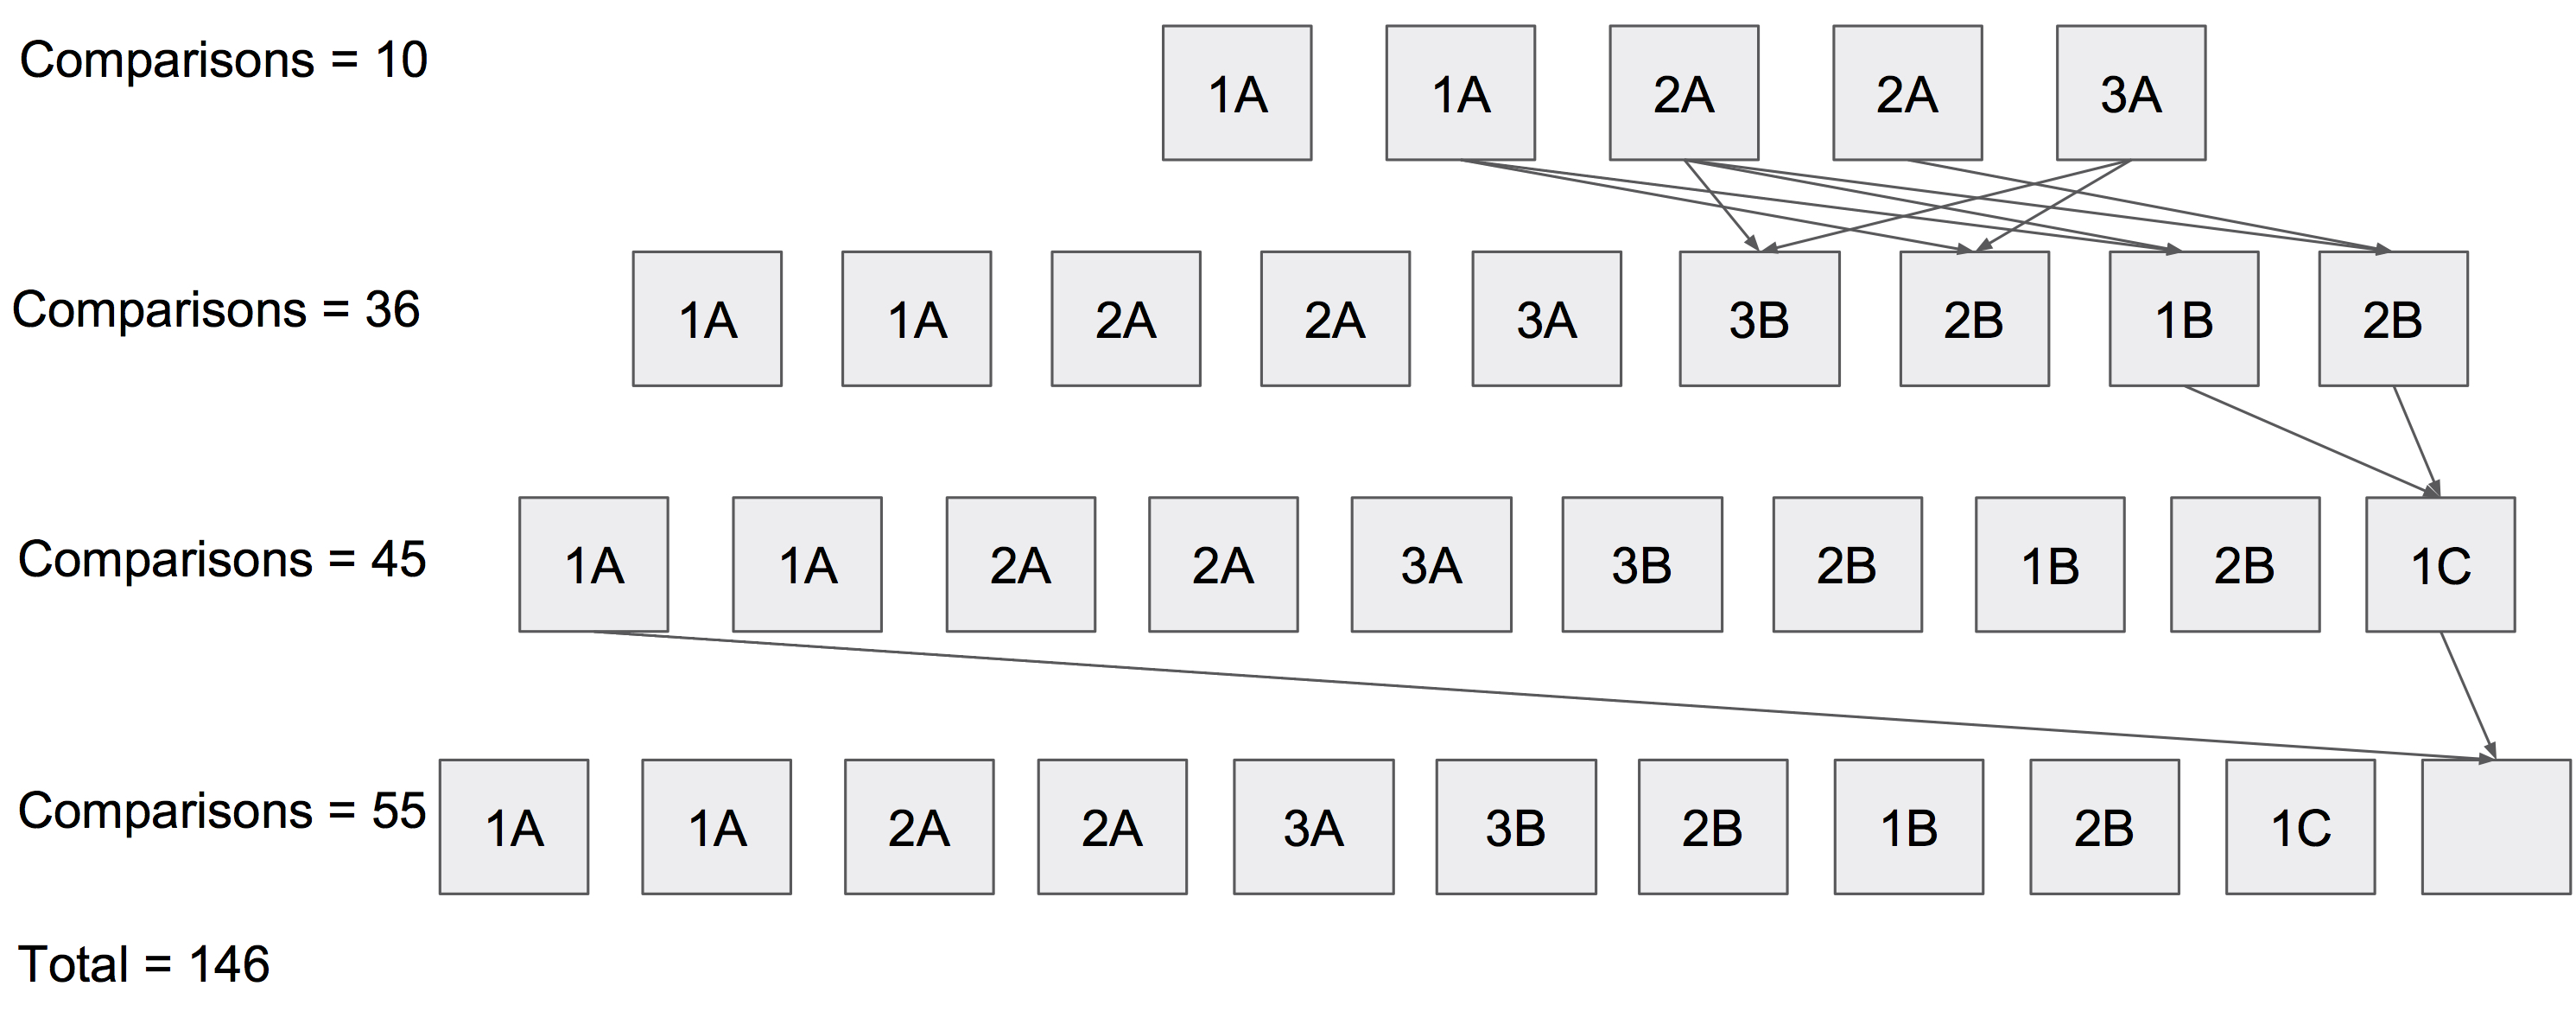
\includegraphics[scale=.084]{ClassicDiag}
  \caption{\textbf{Classic resolution:} This is an example of classic resolution.  Each box represents a clause and has a number and a letter.  The number represents the number of literals in that clause and the letter represents the pass in which that clause was resolved.  Each row is a pass through the clauses and the lines show which clauses resolve together.  On the left is a count of comparisons, where the number of resolutions in each pass is counted.  You can see that every clause is used in every pass and it takes 4 passes to reach the empty clause.}
\end{figure}

\begin{figure}
  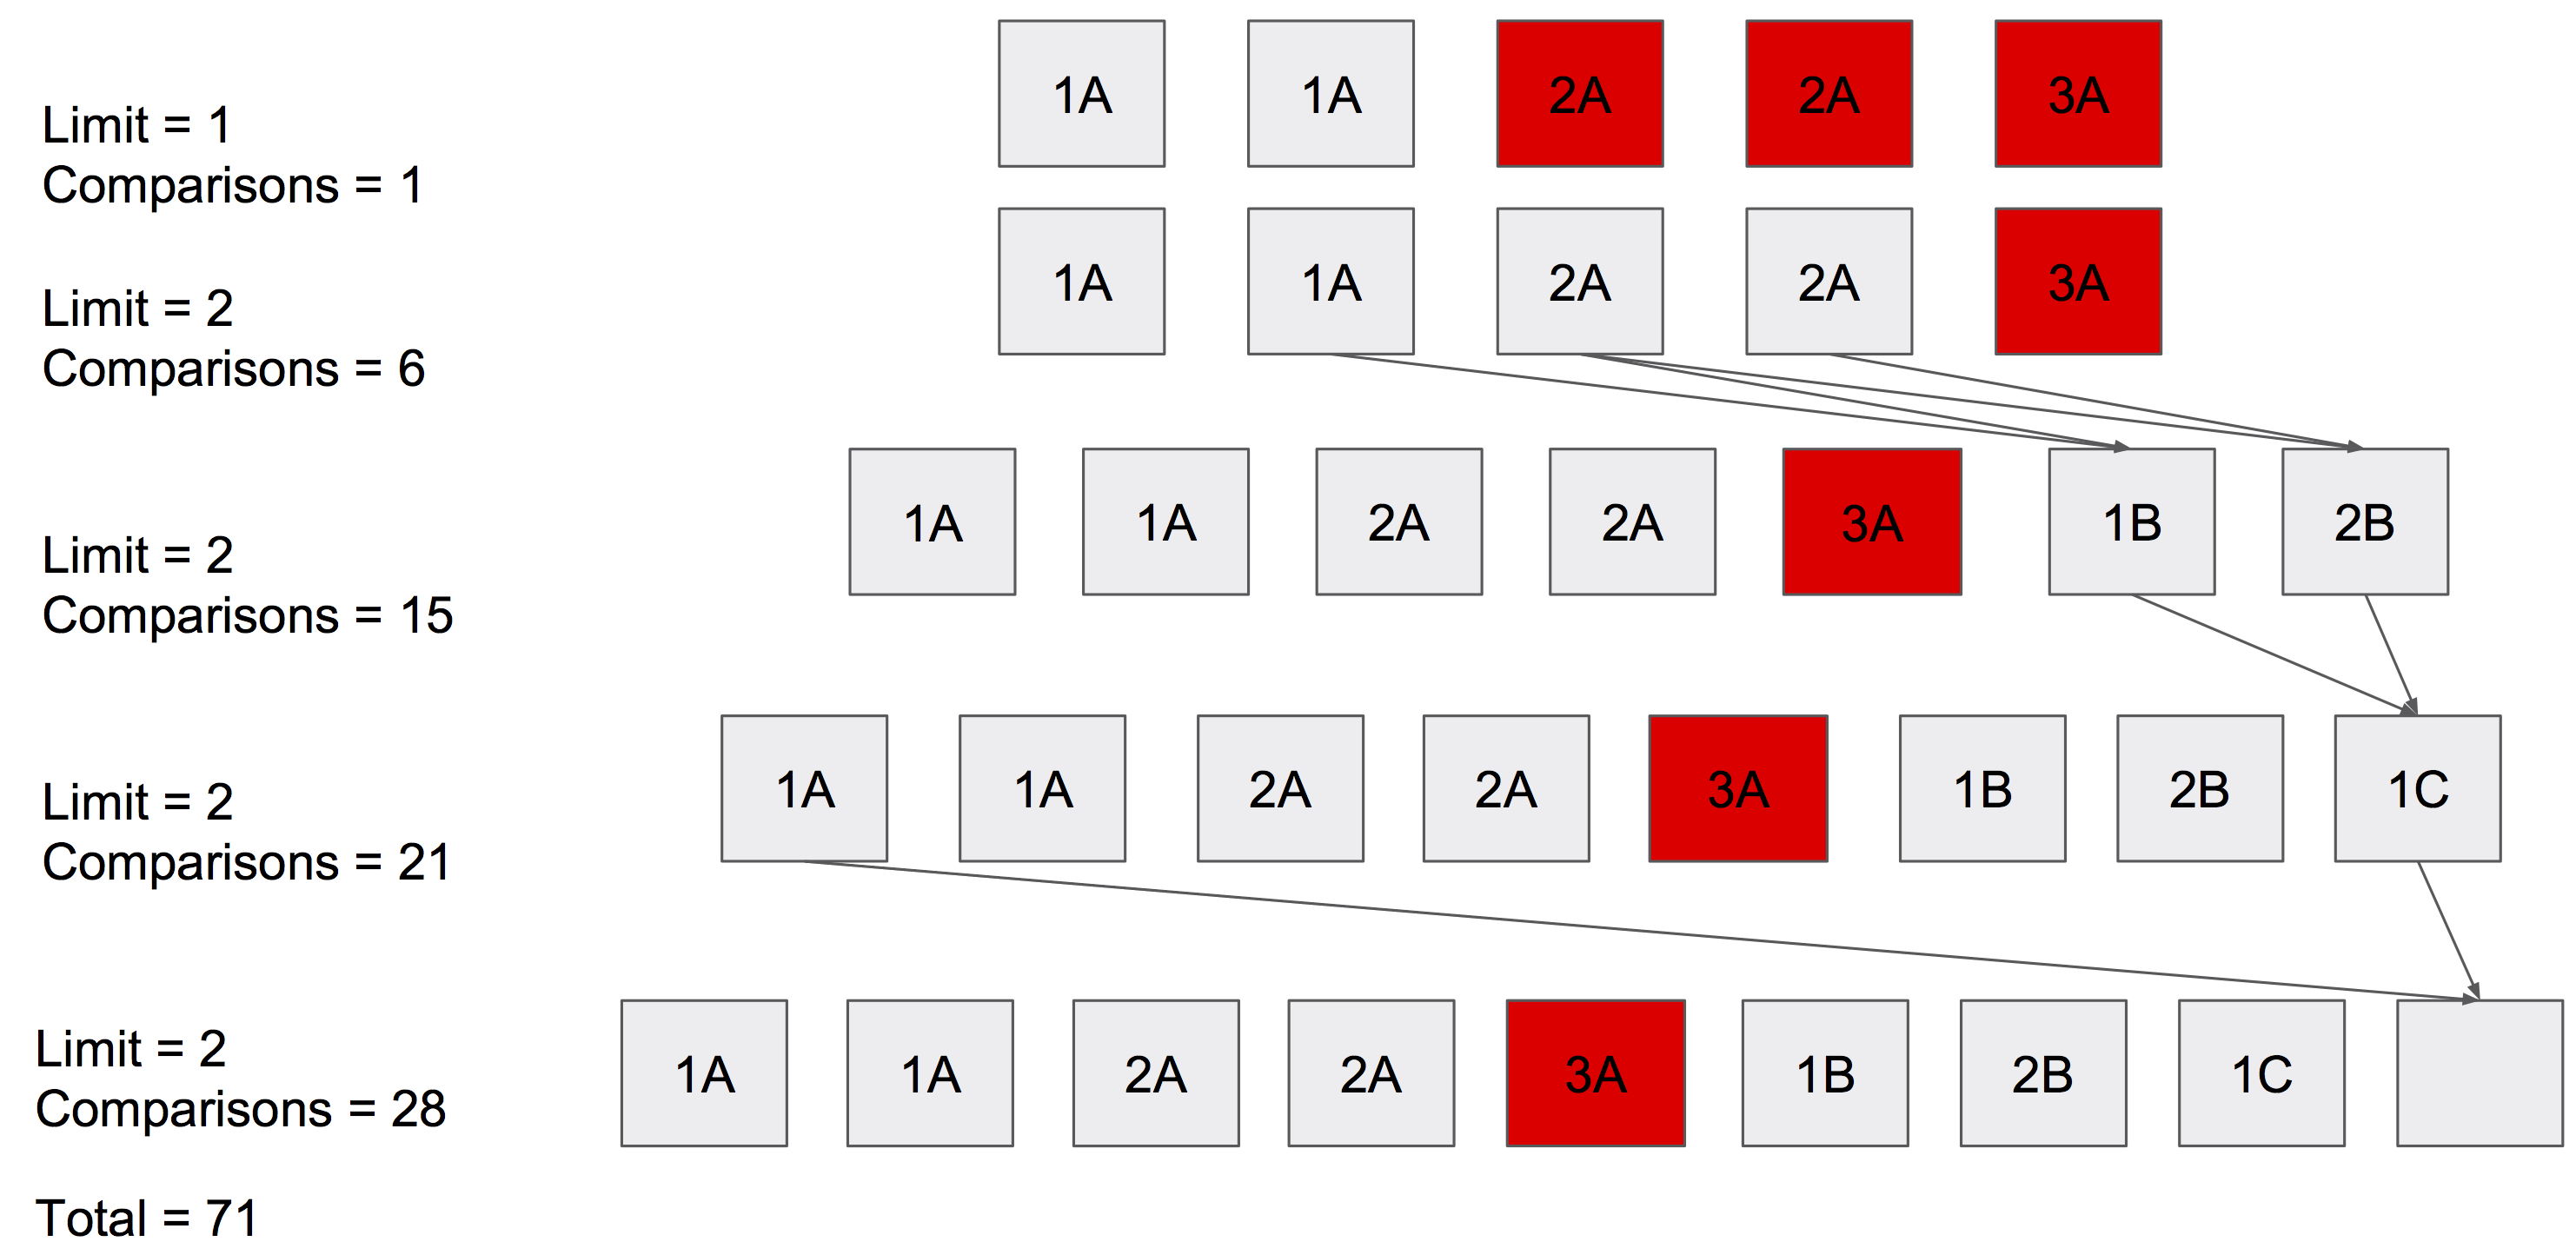
\includegraphics[scale=.084]{IterativeDiag}
  \caption{\textbf{Iterative resolution:} This is an example of iterative resolution.  The red boxes represent clauses that are not being used in that pass of resolution because they have too many literals.  The number of literals being allowed in each clause is shown as the limit to the left of each row.  In this case not every clause is used before the empty clause is found and it takes 5 passes through the clauses.}
\end{figure}

\subsection{Knowledge Base Generation}

Because we were unable to find a dataset of knowledge bases and queries, we had to generate our own.  Our Method of generating knowledge bases was fairly simple.
\begin{enumerate}
\item Generate a new clause randomly
\item Resolve that new clause with the KB
\item If the empty clause is found, go back to step 1
\item If not, add the clause to the knowledge base	
\end{enumerate}

A knowledge base must be consistent.  This is why step 3 goes back to step 1 when the empty clause is found.  This process depends largely on the random clauses that are generated.  As the knowledge base gets larger it become more and more difficult to generate a random clause that is consistent with all the previous clauses.  We found that even generating a knowlegde base with 8 clauses can take over 1000 clause generations.

Because it takes so many resolutions to generate a single knowledge base, we had to limit the amout of time we were willing to wait so the testing could complete in a resonable amount of time.  We decided a resonable amount of time to wait was 5 seconds.  After 5 seconds the generation was terminated and a new one began.  This process inherently filters the composition of our knowledge bases.

We are unsure exactly what type of bias this introduces into our knowledge bases, but it should favor combinations of clauses that are able to resolve quickly over ones that may take longer.  This is unfortunate because we hypothesised that iterative resolution would have more benefit as the resolution has to go deeper.  We could have waited longer, but There were issues with our implementation of theads that prevented long tests.

\subsection{Threads}

One of the biggest drawbacks with resolution is that when the query is false it must continue until there are no more clauses to resolve.  Each pass through the clauses is exponentially larger than the last, so it not practical to wait for the algorithm to finish.  We needed another way to find if a query was false.

Resolving the complement of the query gets false results much faster.  If the complement of a query is true, the query must be false.  Becuase true results can be found far more quickly, we can resolve the query and resolve the complement and whichever one is true tells us the answer.  There is one case, however, where both the query and its complement will be false.  This can happen if the query is completely unrelated to the knowledge base.  In this case, there is nothing in the database to contradict the query or its complement because they have no similarity, so both resolutions will have to run to the end.  This is largely irrelevant in practical applications.

To implement this we used threads.  We ran the resolution of the query and the resolution of its complement in parallel and once one finished we had our answer.  Once one of the resolutions finished, we terminated the thread for the other resolution and returned the answer.  If the query was unrelated to the knowledge base, we would have to wait for the resolution of the query to end whether the resolution of the complement ended or not.

There were no concurency issues with these threads because they never access the same data.  They both run independently with their own instances of resolution.  However, this does take more memory.  Because we are running resolution twice we use twice as much memory for storing new resolved clauses.  The algorithm isn't fast enough to increase the number of clauses to a problematic level unless it is left running for multiple minutes.  However this does become a problem because we had thead termination issues.

Because threading was not built into the algorithm from the start, we had to use external termination of a thead when the other thread finished.  Termination of threads is very difficult and because there are many different opperations the thread could be doing when termination is called, there is no guarantee that it will be successful.  We found that when conducting tests with tens of thousands of resolutions, many threads would fail to terminate and continue resolving.  This means that they continue to increase the number of resolved clauses and take more and more memory.  Especially once 10 or 20 threads failed to terminate, memory starts to become a big issue as well as time.

These failed terminations take up much of the execution time once they start piling up.  It quickly slows the testing down to the point where single resolutions can take minutes instead of seconds.  This is why we could not conduct longer tests.  We often had to end tests when too many threads failed to terminate, and having to do that when tests take much longer is unrealistic.

\section{Evaluation}

Testing involved two steps, first a knowledge base was generated, then a query was generated and resolution was timed.  As stated above, knowledge base generation had to be limited to 5 seconds.  We did the same for timing the query resolutions.

We chose 5 seconds as a reasonable amount of time for a query to resolve.  This too inroduces a bias toward queries that resolve faster.  It is difficult to tell what effect this bias has but we can speculate.  Iterative resolution is targeting resolutions that require more passes through the clauses.  Because the number of clauses grows exponentially, Standard resolution quickly reaches a pass where it will take an unreasonable amount of time to finish.  Iterative resolution spreads those resolutions out into multiple passes so that the algorithm can hopefully get to a deeper level where the solution is.  We may be testing The algorithm in an environment where its benefits are unable to be seen.

We tests different amounts of clauses, constants, and functions.  We did a minimum of 20 trials for each test,  and tested at most 5 queries on any one generated knowledge base.  We also always used the same queries for both alrogithms, so they are tested on the exact same data.  We report the number of processor cycles needed to complete each resolution as our measurement of speed.


\begin{figure}
  \begin{center}
    \begin{tabular}{|c|r|r|}
      \hline
      Clauses & Classic & Iterative \\ 
      \hline
      3 & 7031615 & 10103252 \\
      4 & 9925390 & 11892015 \\
      5 & 11585391 & 14429799 \\
      6 & 6910083 & 8153731 \\
      7 & 20839983 & 28055736 \\
      8 & 10660459 & 14018322 \\
      10 & 9165610 & 26490492 \\
      15 & 19339043 & 34255509 \\
      30 & 79460615 & 85667340 \\
      \hline
    \end{tabular}
  \end{center}
  \caption{Average number of cycles taken at each quantity of clauses for classic and iterative resolution.}
\end{figure}

\section{results}

Our tests revealed very little difference between classic and iterative resolution.  We saw the most difference when compared against the number of clauses.  For both algorithms, as the number of clauses increased the cycles taken to resolve increased.  This was unexpected because the algorithm already creates new clauses very quickly, ending up with thousands in the knowledge base after a few passes, so it would seem that starting with a few more shouldn't effect it very much.  We believe this occured because the resolved clauses may be much more related to the knowledge base than a new random clause, so the new random clause is able to create new opportunities for resolution that the clauses that existed before would not be able to get to.

Although both algorithms take longer as the clauses increase, iterative resolution seems to do worse than classic resolution when there are more clauses.  We can see that up until 10 clauses the two algorithms have very similar performance (figure 7).  At 10 clauses iterative resolution becomes worse than classic and stays that much worse up to 15 clauses.  To get a better idea of why this occured we take a closer look at the performance when we fix the number of constants used.

\begin{figure}
  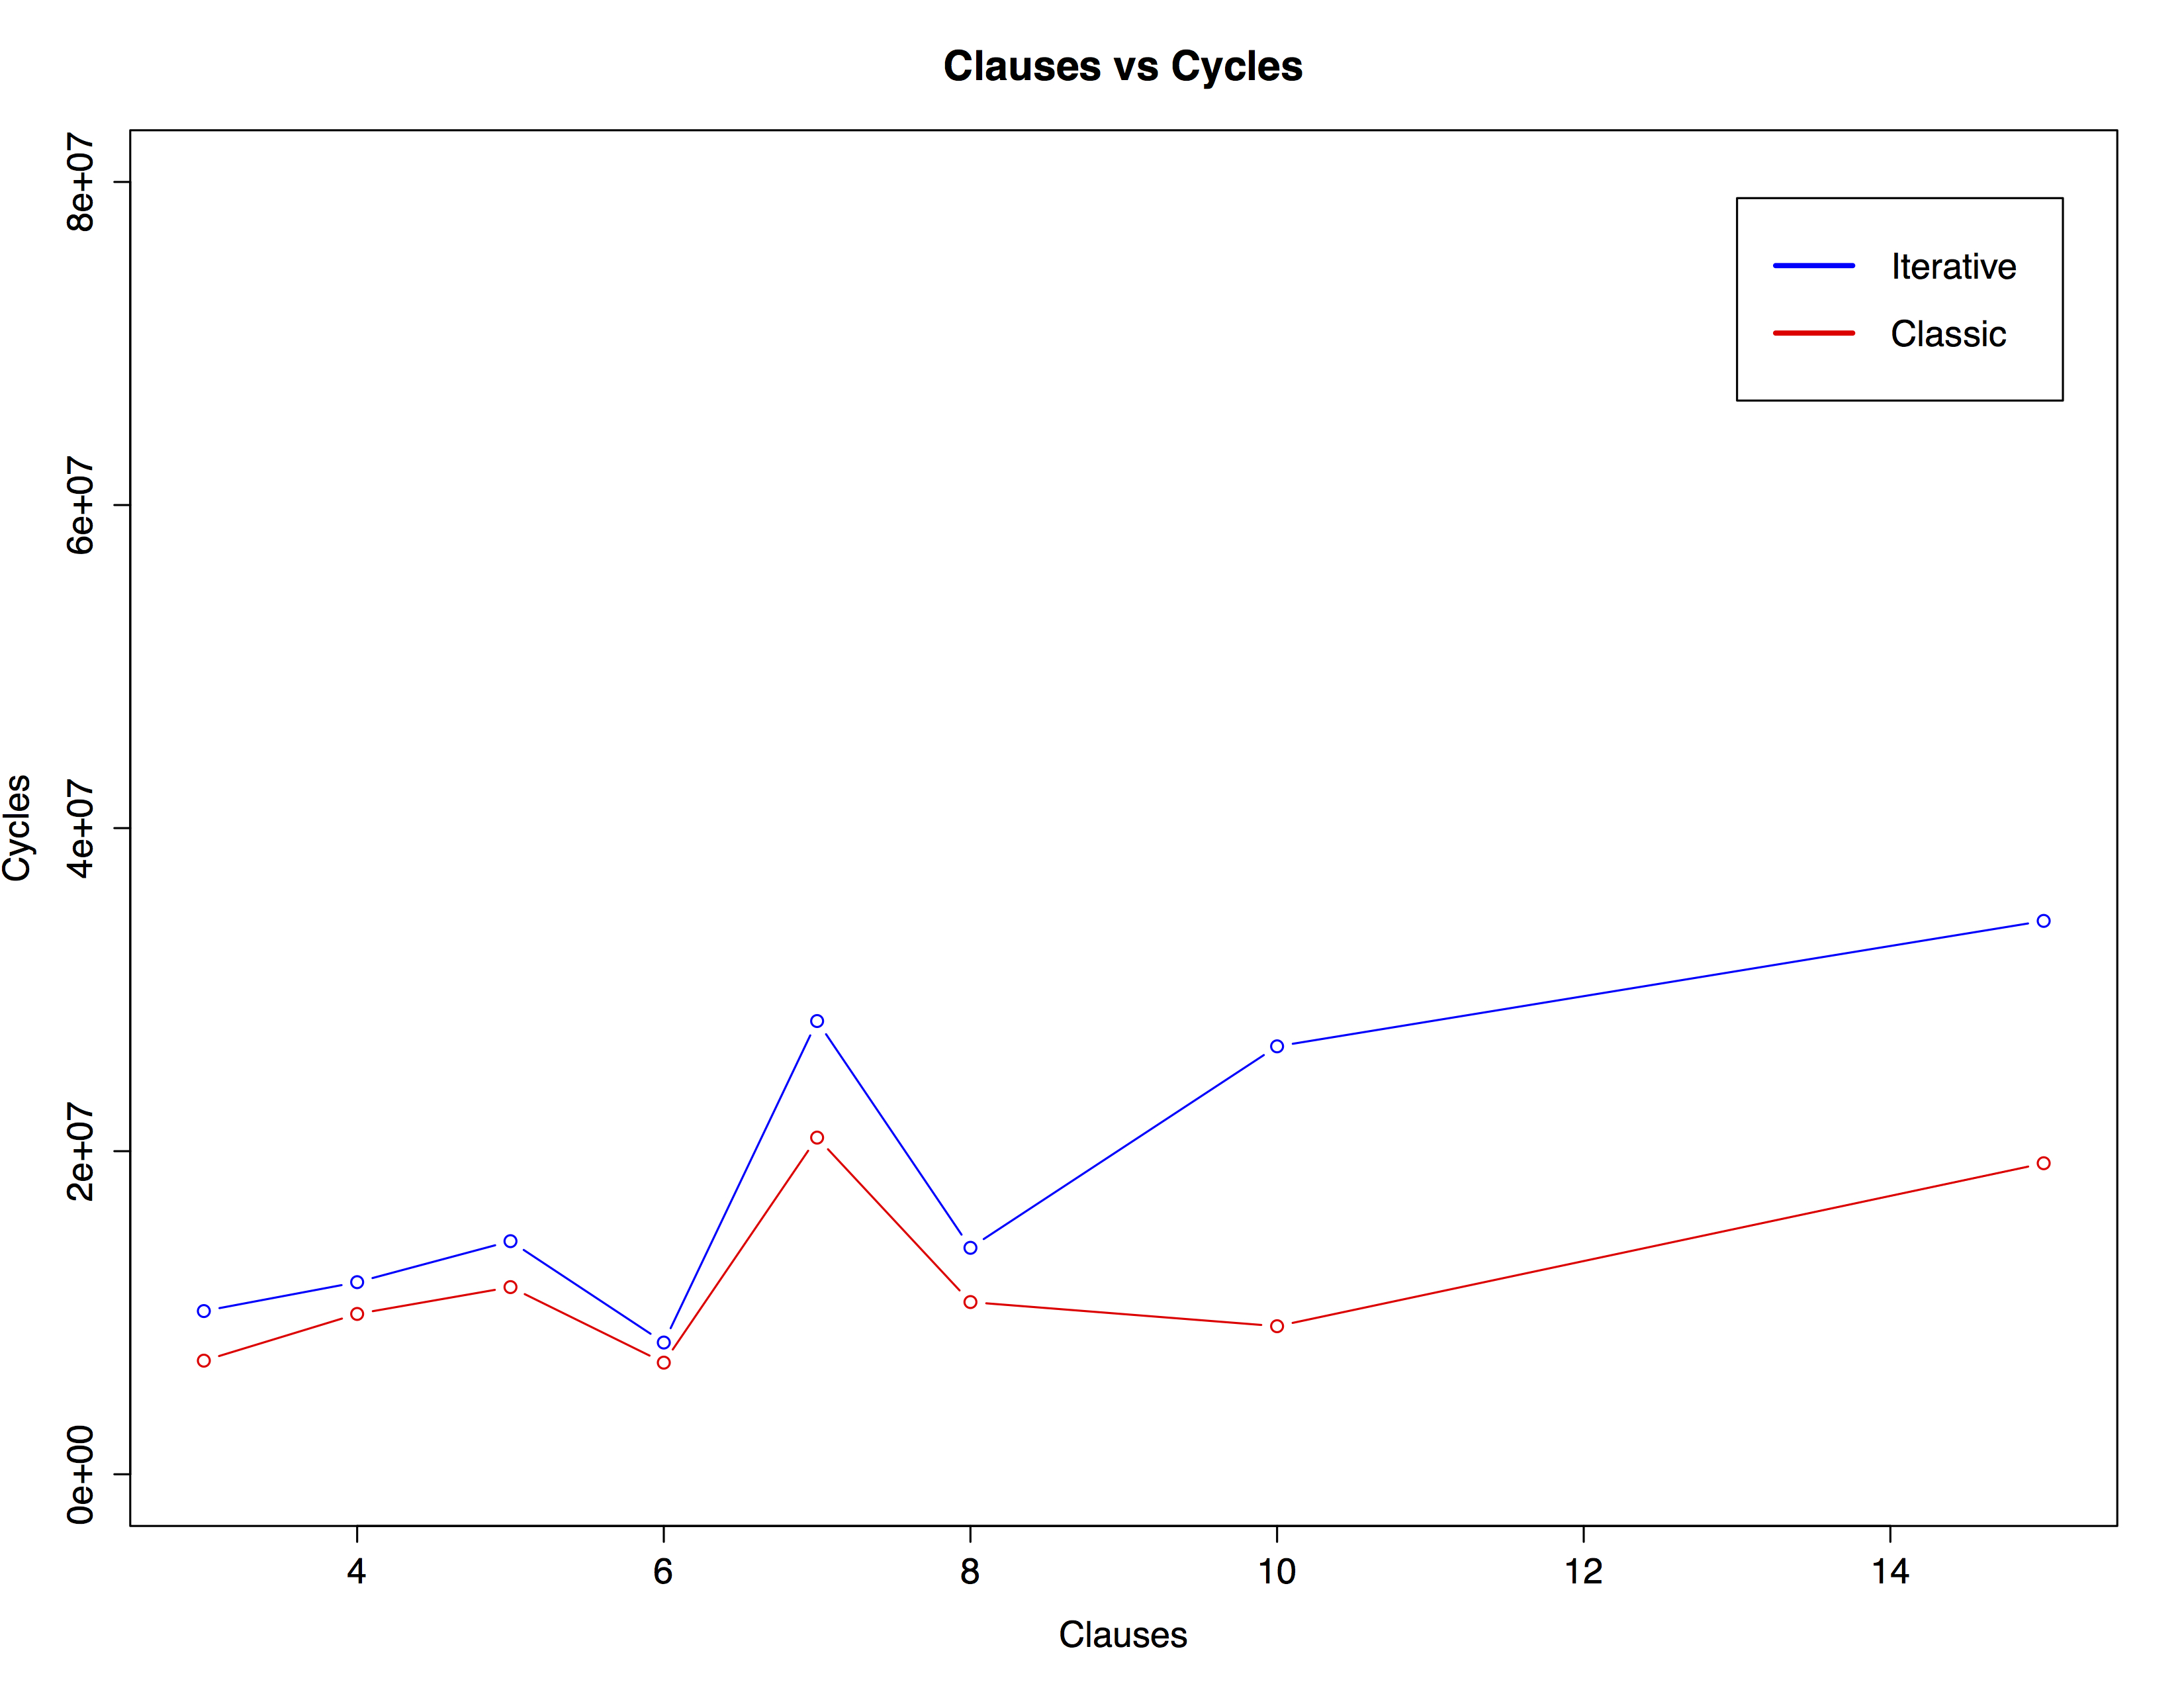
\includegraphics[scale=.078]{Clauses}
  \caption{Graph of cycles taken to resolve knowledge bases from 4 to 15 clauses.}
\end{figure}

When the number of constants is fixed below 3, both algorithms perform very similarly all the way up to 15 clauses.  When the number of constnats is fixed at 3 (figure 8) We see a very similar shape to the graph in figure 7 with a more accentuated spike at 7 clauses.  The decrease in performance for iterative resolution at 10 clauses is nearly identical.  When constants is fixed at 4 (figure 9) There is a much more dramatic decrease in performance for iterative resolution at 10 clauses.  Inerestingly it performes better at 15 clauses than at 10, but it still takes far more cycles than with lesser numbers of constants.  This suggests that the difference we see in the overall performance of different clause lengths in figure 7 comes from the datapoints where there are more constants.

We see a similar trend when we fix the number of functions.  With low numbers of functions the two algorithms perform very similarly, but when the number of functions is fixed at 4 we see a dramatic decrease in performance for iterative resolution at 10 clauses.  This is similar to the decrease in performance as the number of constants increased, but at 15 clauses the performance returnes to being just as good as classic resolution.  This is very strange behavior and is something we would like to look into further in future testing.  Althrough the performance is comperable at 15, the spike at 10 likely causes some of the overall performance loss as clauses increase.  


\begin{figure}
  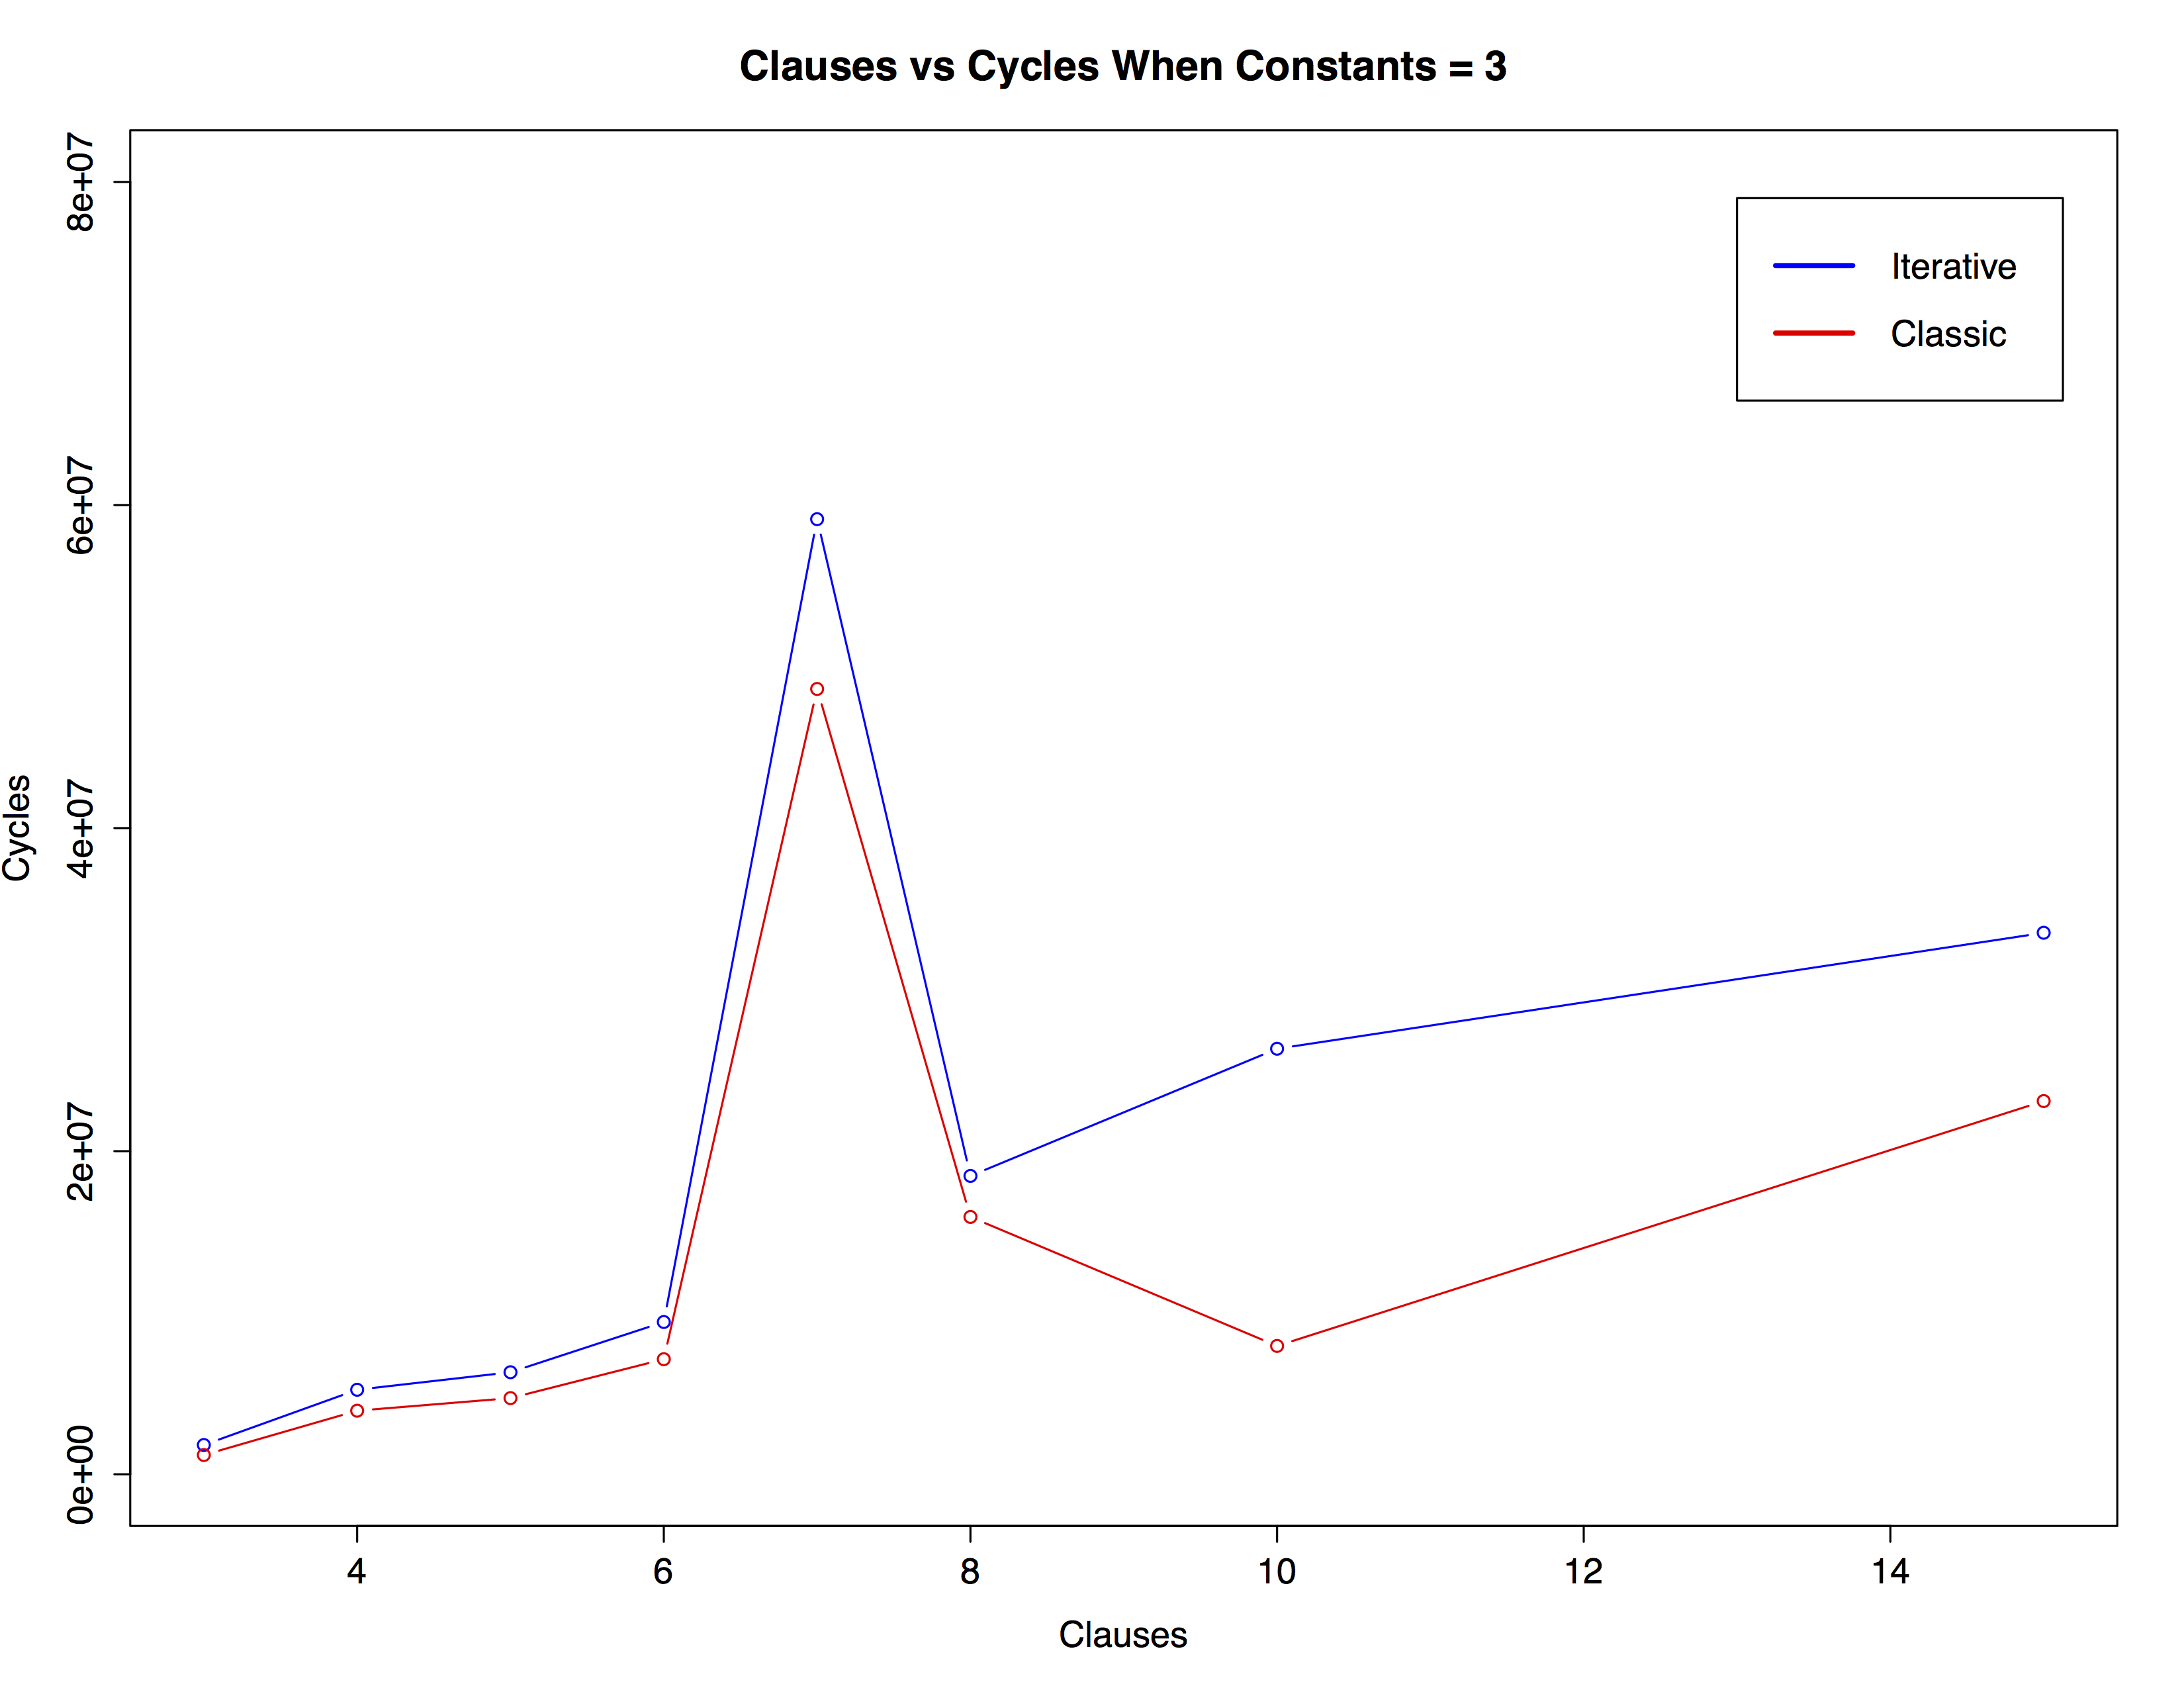
\includegraphics[scale=.078]{ClausesConstants=3}
  \caption{Graph of cycles taken to resolve knowledge bases from 4 to 15 clauses when the number of constants is fixed at 3.}
\end{figure}


\begin{figure}
  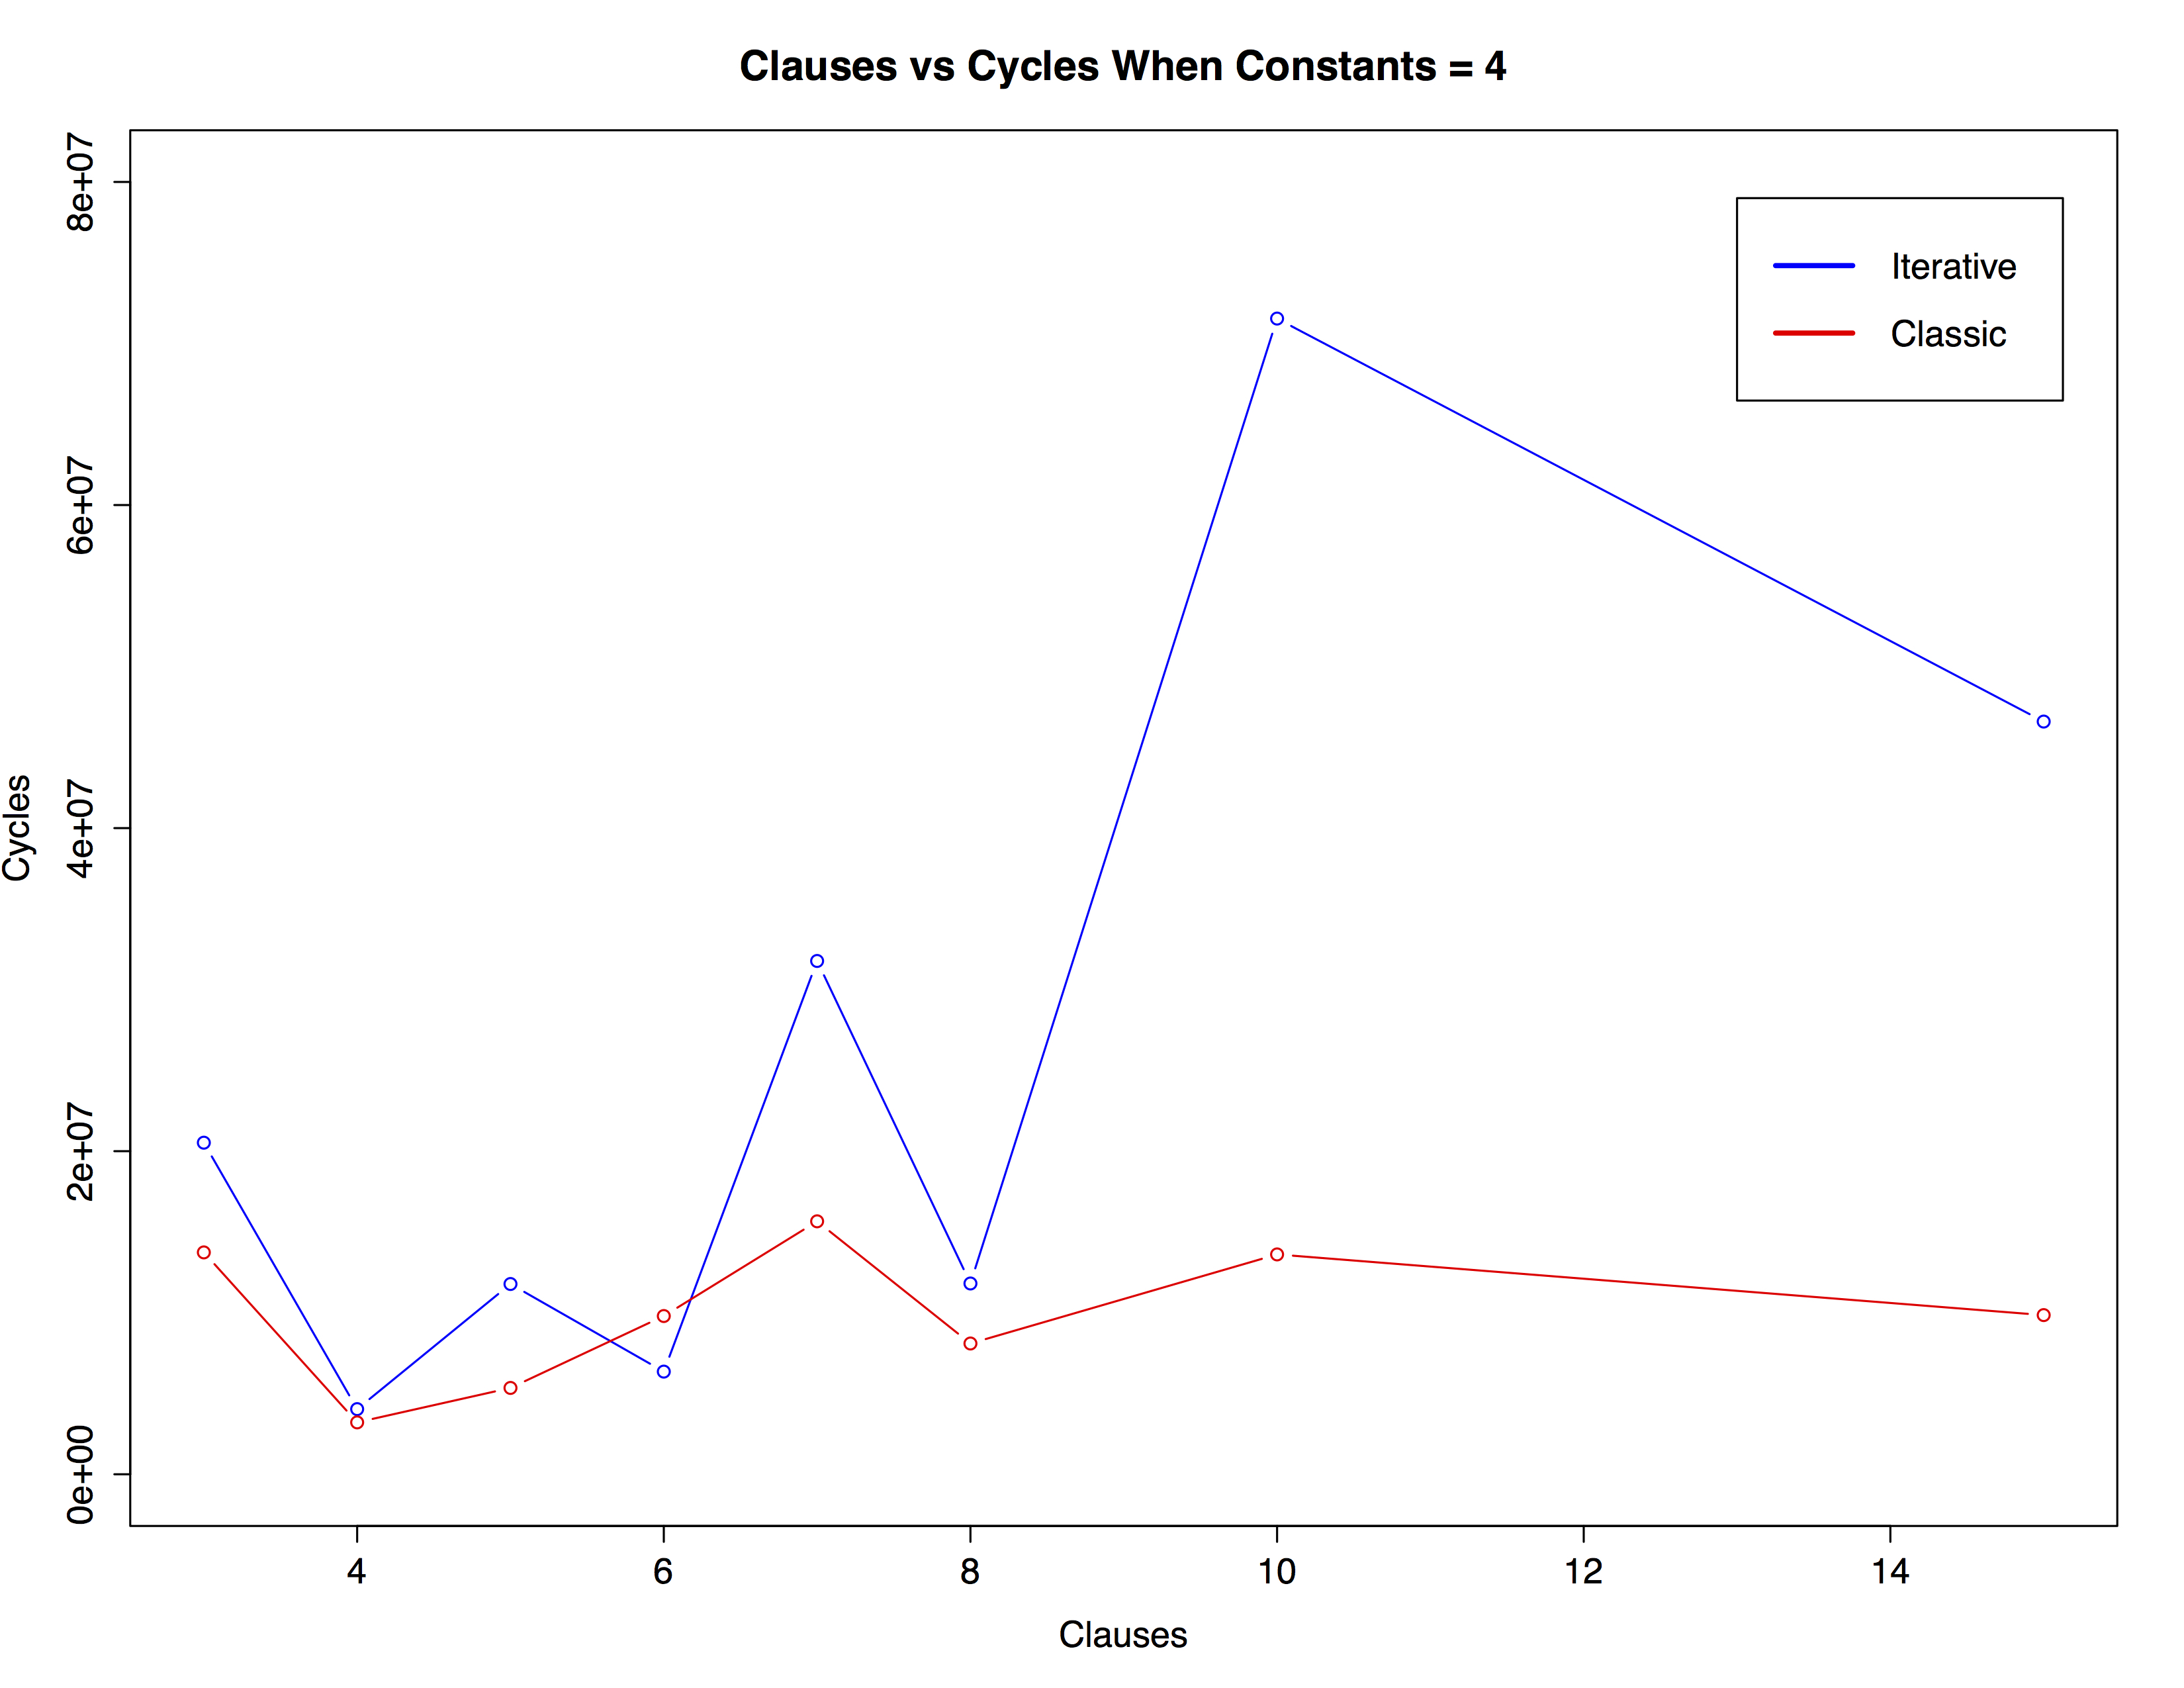
\includegraphics[scale=.078]{ClausesConstants=4}
  \caption{Graph of cycles taken to resolve knowledge bases from 4 to 15 clauses when the number of constants is fixed at 4.}
\end{figure}

The two graphs comparing the speed with different numbers of functions and constants show a constant trend (figure 11,12).  Both functions and constants have very little effect on the time it takes to resolve overall.  We assumed these would have a greater effect because with more functions and constants unification becomes more complicated.  We may not have a large enough range to see a trend but because of time constraints we were unable to go further.  For both iterative and classic the trend is the same, but classic is always slightly faster than iterative.

Although there is no trend overall, we already saw that when there is a high number of clauses and a high number of constants or functions the cycles increase dramatically.  This suggests that with low numbers of any of these variables, resolution is able to complete fairly easily and doesn't produce much difference between the algorithms, but when multiple have high numbers, resolution becomes much harder for the iterative algorithm.

All of these results show classic resolution increasing steadily as the number of constants, functions, or clauses increases.  Classic resolution has small spikes in bad performance.  On the other hand, iterative resolution has large spikes in bad performance and the performance decreases rapidly as the values of constants, functions, or clauses gets large.  This is the opposite of what we expected.  Assuming these resolutions that are taking longer are at a deeper level in the resolution, we would think that iterative resolution could reach them faster.  We likely need to run the testing differently to get more accurate results.

Even though we had hundreds of datapoints for each of the averages in these graphs, it is likely that the data still has not converged.  The standard deviation for all of the averages is from 70 to 120 billion.  The averages only range from 7 to 80 billion, so we cannot say with certainty that any of these trends represent the actual behavior of the algorithms.  None of our results are significant enough to distinguish one algorithm as better than the other.  To fix this we will have to run many more trials and try to increase the range of our variables to see a larger trend in the data. 

\begin{figure}
  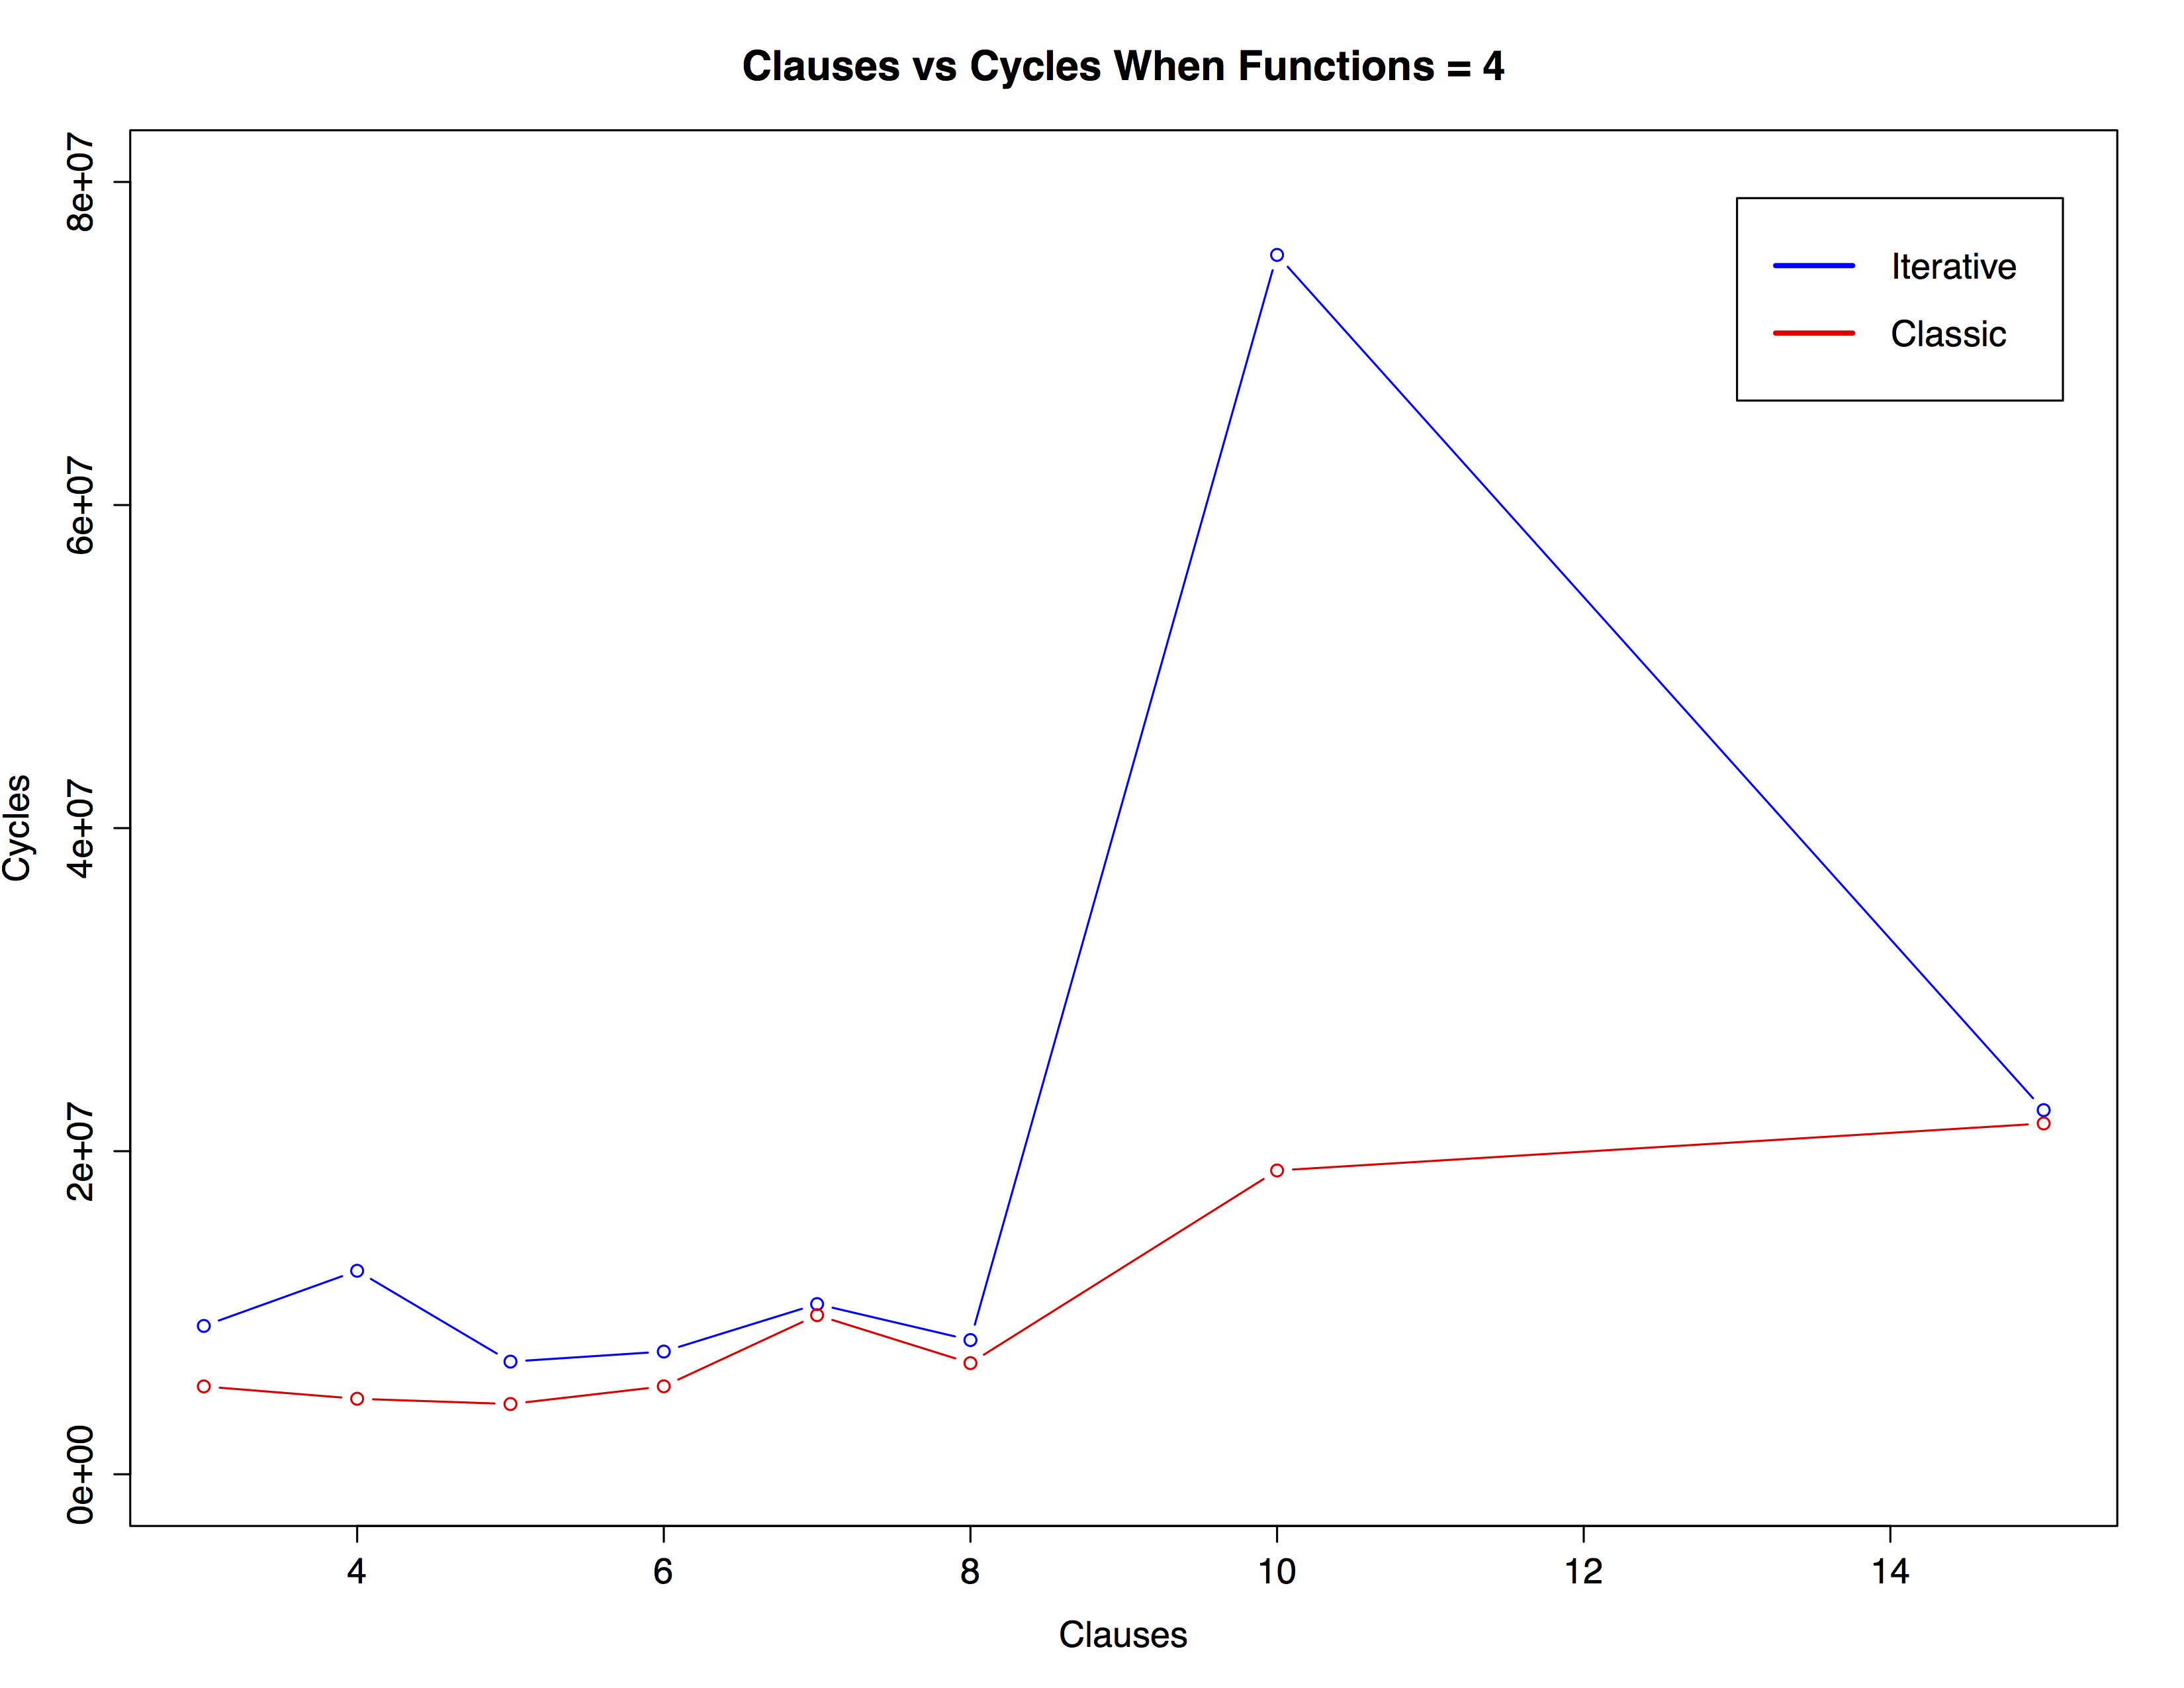
\includegraphics[scale=.078]{ClausesFunctions=4}
  \caption{Graph of cycles taken to resolve knowledge bases from 4 to 15 clauses when the number of functions is fixed at 4.}
\end{figure}

\begin{figure}
  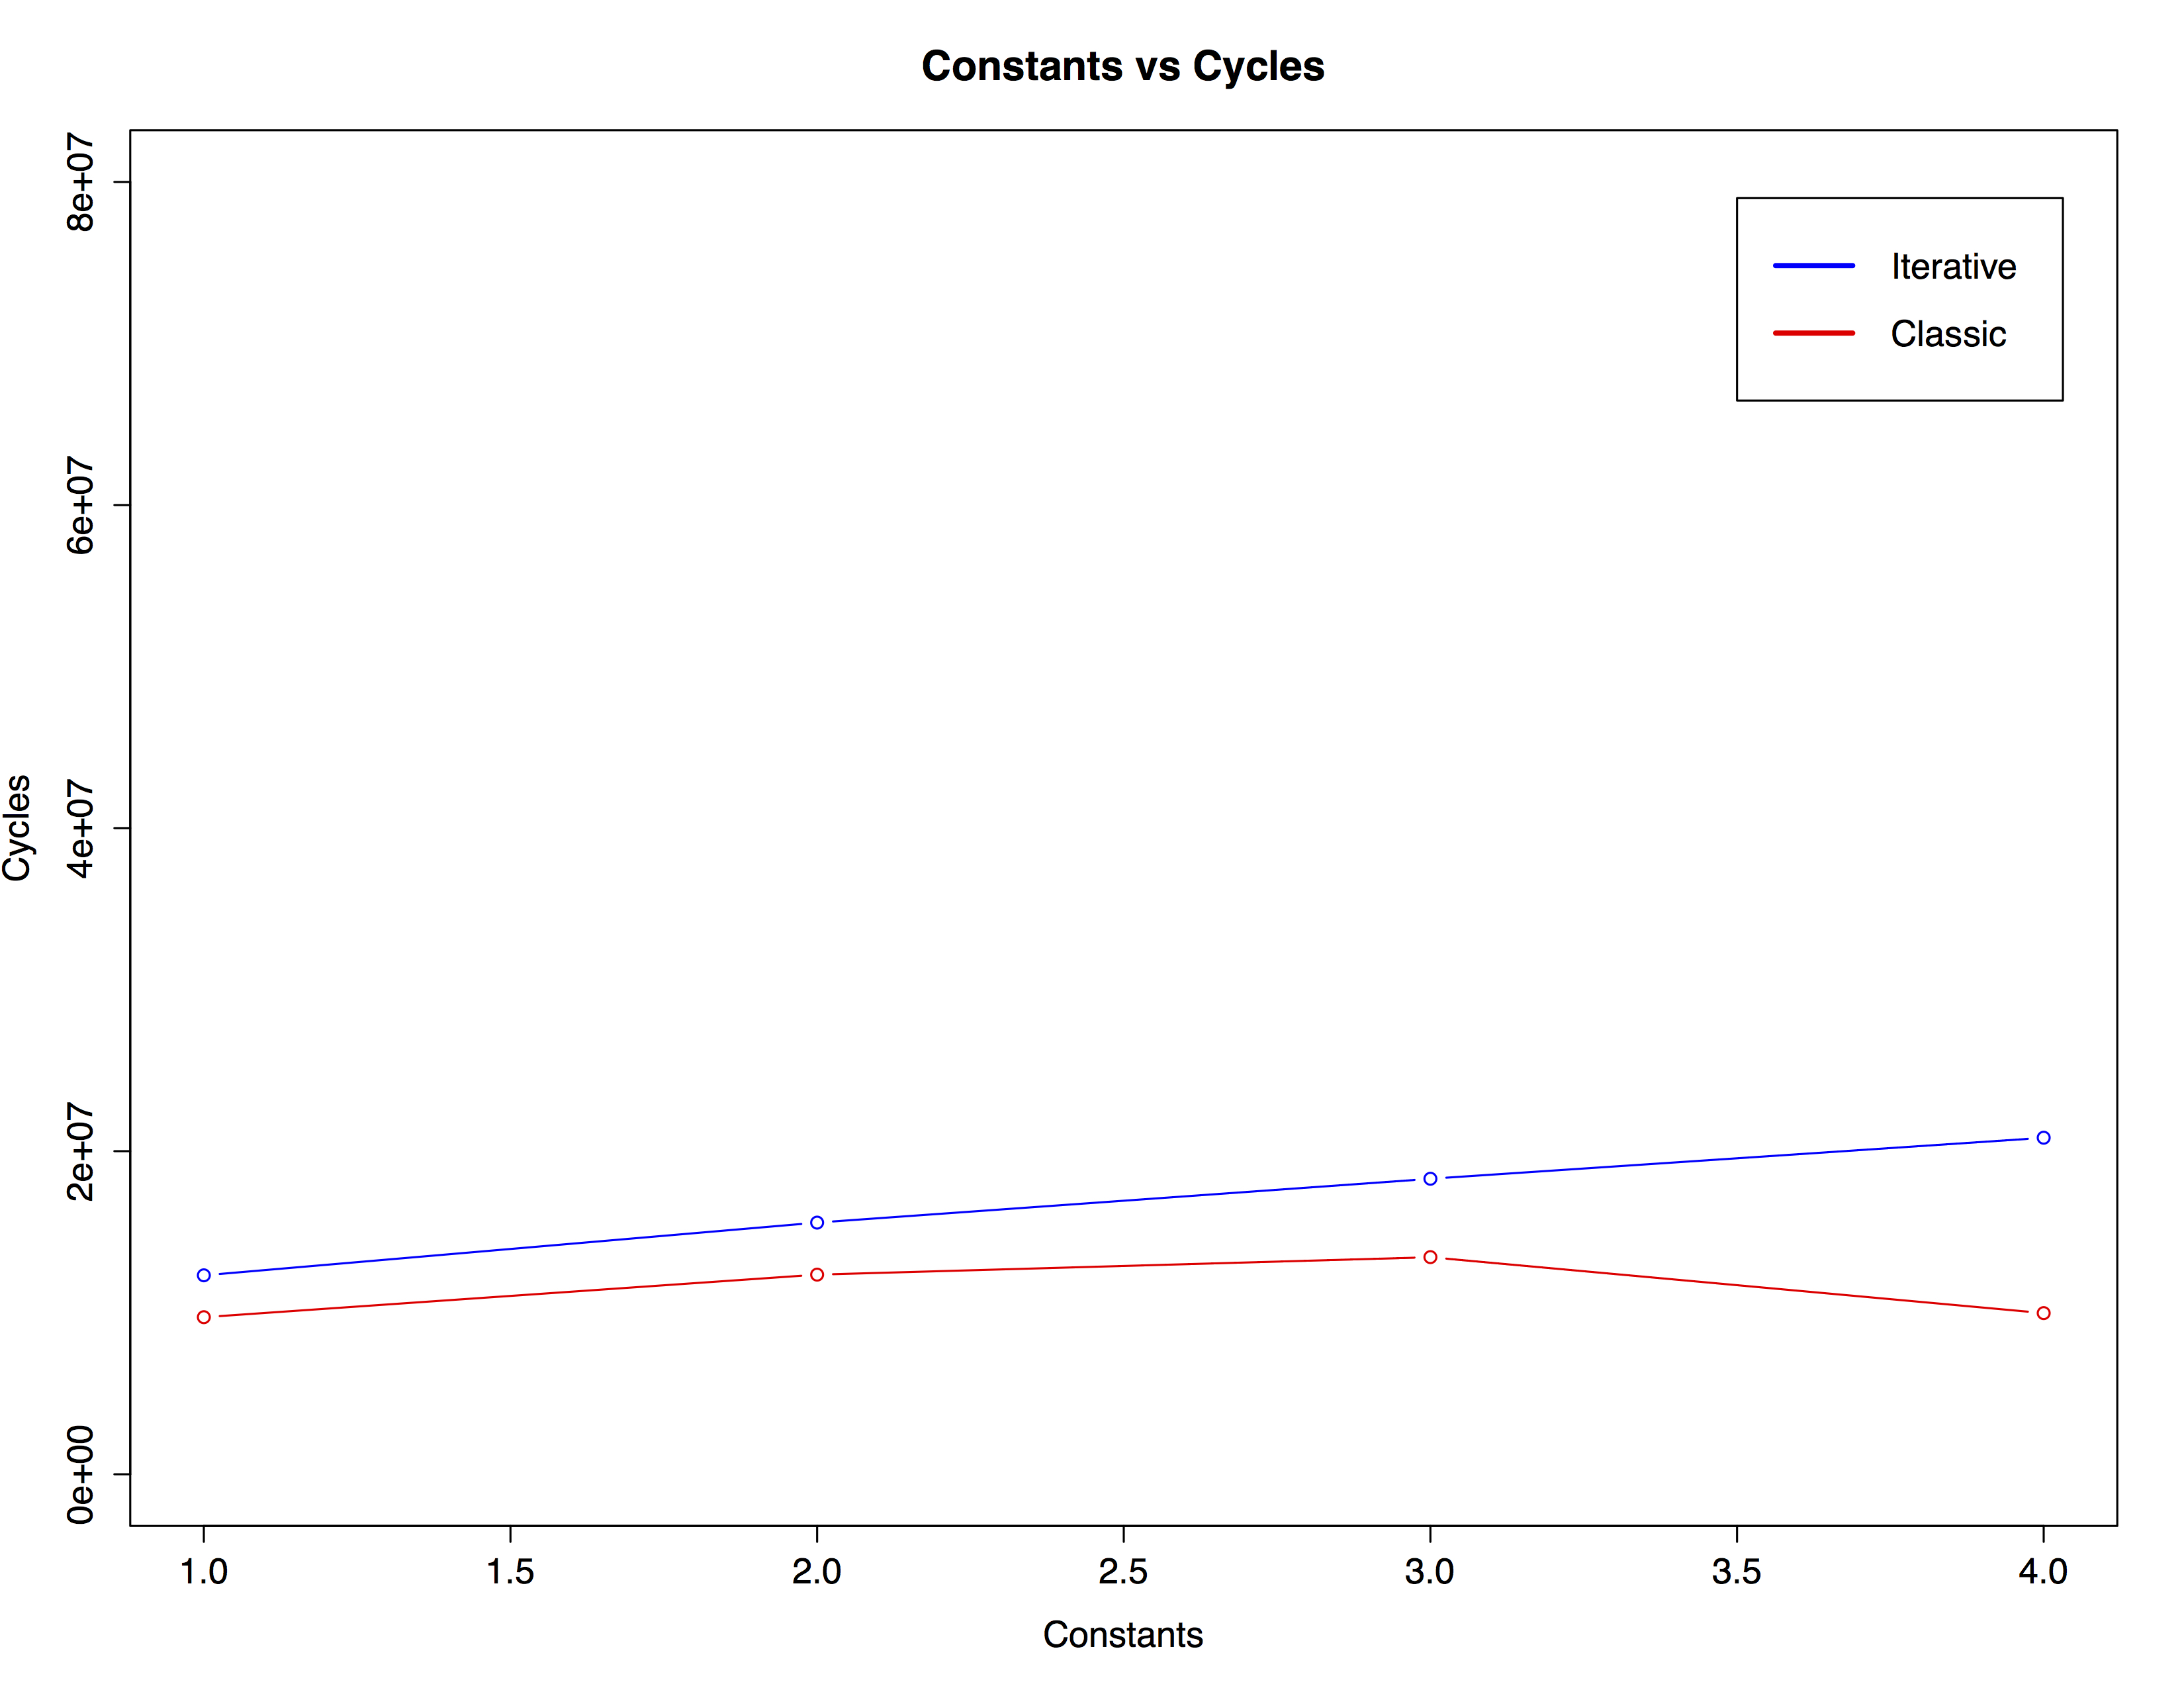
\includegraphics[scale=.078]{Constants}
  \caption{Graph of cycles taken to resolve knowledge bases from 1 to 4 constants.}
\end{figure}

\begin{figure}
  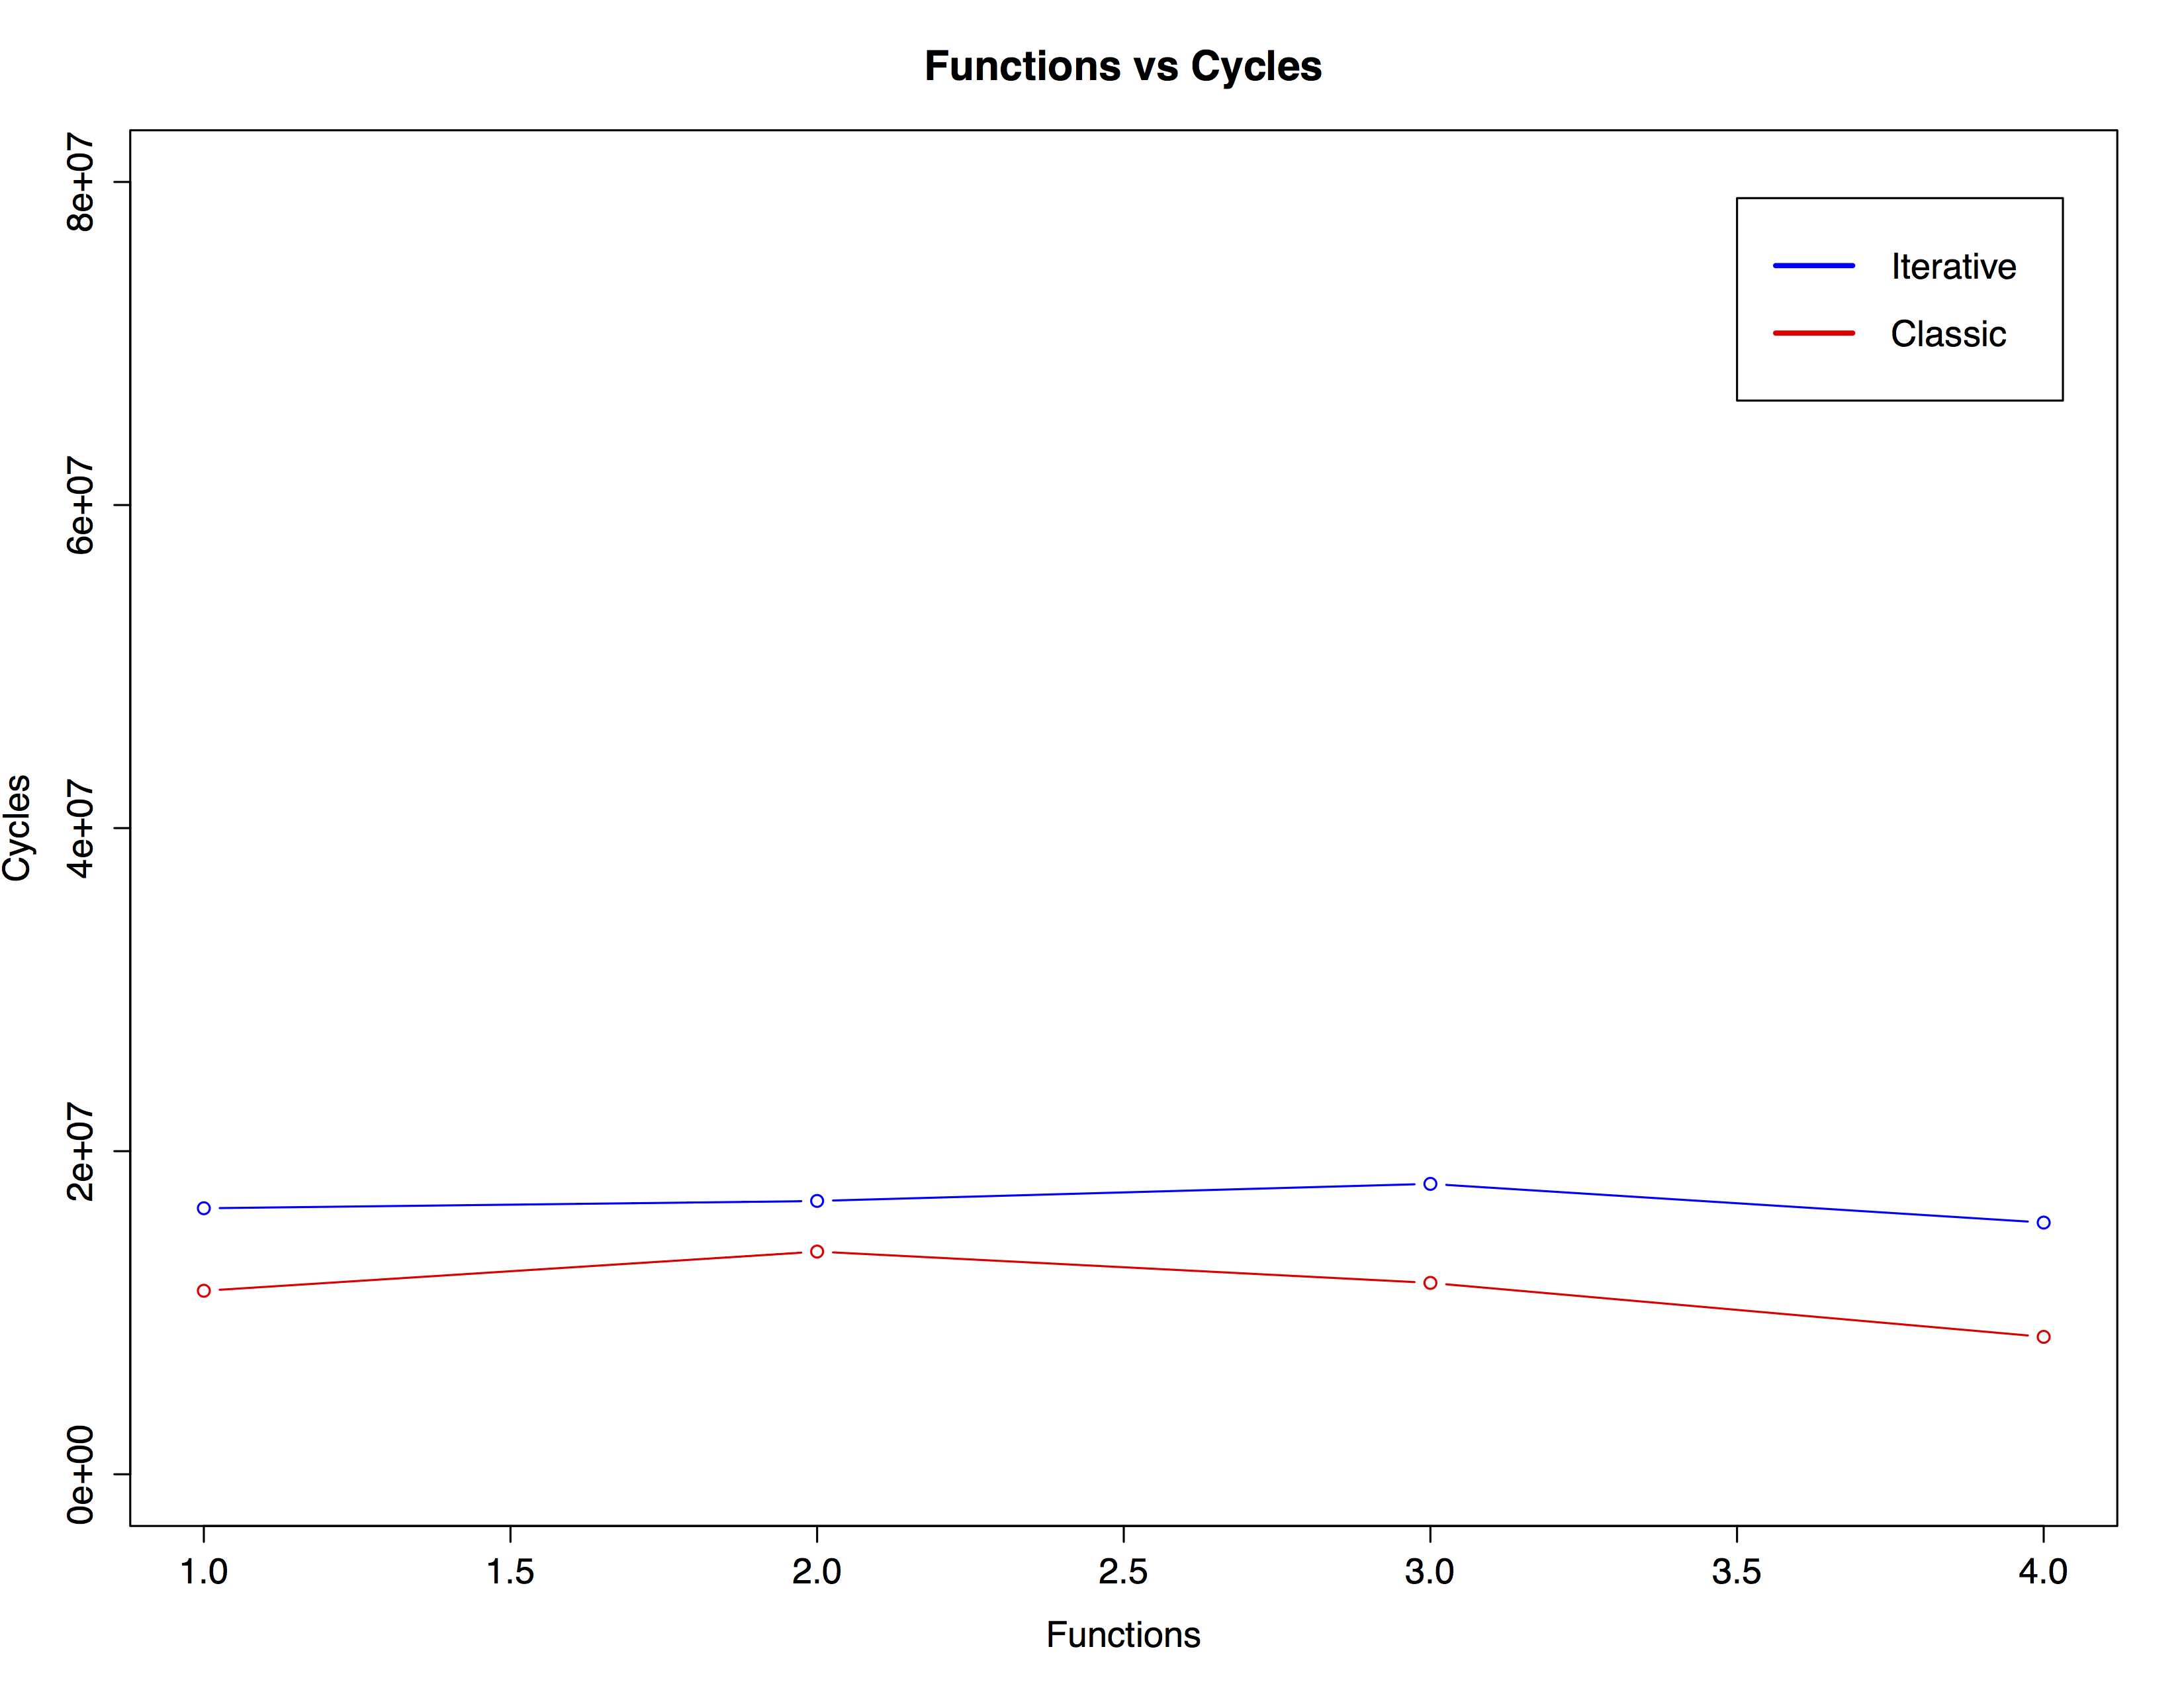
\includegraphics[scale=.078]{Functions}
  \caption{Graph of cycles taken to resolve knowledge bases from 1 to 4 functions.}
\end{figure}

\section{Conclusions}

Iterative resolution does not improve the resolution algorithm.  It was outperformed by classic resolution in all tested quantities of clauses, constants and functions.  The results were not significant enough to show that one was better than the other, but on average iterative resolution does not offer any improvements.  For future research it would be worth modifying the algorithm to avoid repeating resolutions it has done on previous passes.  This could avoid much of the drawback associated with iterative resolutions, which is that it does more passes and everything is reresolved on each pass.  Alternatives to threads are also necessary, such as a self regulating termination after a certain time has elapsed within the resolution method itself.
\section{Future Directions}

\subsection{Threads}
Much of the data we collected suggests that the interesting differences between these algorithms are present when the values of clauses, functions, and constants are high.  The primary issue to confront next is fixing the threading issues with the algorithm.  By building thread termination into the code of the algorithm itself, it is possible to eliminate the issue of failed terminations we were unable to do this due to time, but it can be done and would simplify testing tremendously.

Without bugs in threading we would be able to run much larger tests without worrying about failed terminations slowing down the testing.  We could be confident that the larger tests would finish and therefore could do more trials as well as a larger range of variables.  We could also have a much longer waiting time for knowledge base generation, which would hopefully give us less bias in our knowledge bases.

\subsection{Real World Testing}

Another important directions would be testing our algorithm on real world problems.  Real world knowledge bases and queries likely have a more organized structure which gives them a particular bias that our algorithm may or may not be better at.  Randomly generating knowledge bases and queries allows us to run much larger tests, but we cannot be certain how useful our algorithm is until we have tested it on real problems.  

\subsection{Data}

Besides collecting more trials and a larger range in our variable, we should collect data from the algorithm itself.  It would be very helpful to know the number of clause resolutions done or the number of literals that were compared in and entire resolution.  This would give us a more accurate sense of which alrogithm is doing more work.  The tool we used to capture the run time is fairly rudementary and could be a large source of variance in our data.  We are unsure of its accuracy and were unable to record some results due to inconsistencies in its output.  By counting the number of basic operations the algorithm is executing, either resolutions or literal comparisons, we would have an exact number for the amount of work the algorithm is doing.

Time is still important because with unification not all literal comparisons take equal time or work, but it is a very good basic measurement to see if our algorithm is doing what we want it to do, which is reduce the number of clause resolutions needed to reach the empty clause.

It would also be good to record the number of passes the resolution made before it found the answer.  This would allow us to see if our theoretical reason for why interation should be faster is true.  We believe iteration should be faster because it can reach a deeper level in the resolution tree (make more passes) faster.  Therefore, we would like to be able to see if iterative resolution does better when the resolution has to go deeper.  This would also give us insight into why the results we see seem to be the opposite of this theoretical improvement.  

\section{Acknowledgments}
I would like to thank Matthew Whitehead and Steven Janke for their guidance and support with this research.  I would also like to thank the Colorado College  Mathematics and Computer Science Department for all the support and opportunity it has given me throughout my college career. 

\bibliography{BibResolution}
\bibliographystyle{plain}

\end{document}
